\documentclass[12pt,a4paper]{article}
\usepackage[utf8]{inputenc}
\usepackage[spanish]{babel}
\usepackage{amsmath}
\usepackage{amsfonts}
\usepackage{amssymb}
\usepackage{graphicx}
\usepackage{float}
\usepackage{listings}
\usepackage{listingsutf8}
\usepackage{xcolor}
\usepackage{hyperref}
\usepackage{booktabs}
\usepackage{array}
\usepackage{longtable}
\usepackage{fancyhdr}
\usepackage{setspace}
\usepackage{caption}

\usepackage[backend=biber,style=numeric,sorting=nyt]{biblatex}

% Configuración para reducir el tamaño de los captions
\captionsetup{font=small}

% Configuración para reducir espacio en figuras
\setlength{\textfloatsep}{10pt}
\setlength{\floatsep}{10pt}
\setlength{\intextsep}{10pt}

% Configuración de hyperref
\hypersetup{
    colorlinks=true,
    linkcolor=blue,
    filecolor=magenta,      
    urlcolor=cyan,
    citecolor=red
}

% Configuración de listings para código
\lstset{
    basicstyle=\ttfamily\small,
    breaklines=true,
    frame=single,
    numbers=left,
    numberstyle=\tiny,
    keywordstyle=\color{blue},
    commentstyle=\color{green!60!black},
    stringstyle=\color{red},
    backgroundcolor=\color{gray!10},
    extendedchars=true,
    inputencoding=utf8,
    literate={ñ}{{\~n}}1 {á}{{\'a}}1 {é}{{\'e}}1 {í}{{\'i}}1 {ó}{{\'o}}1 {ú}{{\'u}}1 {ü}{{\"u}}1
}

\begin{filecontents*}{bibliografia.bib}
    @article{avila2022,
      author  = {Ávila, Eldo and Martínez, Lucía and Pereyra, Rodolfo and Lang, Timothy and Deierling, Wiebke and Wingo, Matthew and Melo, Gregory and Medina, Bruno},
      title   = {Measurements of size and electrical charges carried by precipitation particles during RELAMPAGO field campaign},
      journal = {Earth and Space Science},
      year    = {2022},
      volume  = {9},
      pages   = {e2022EA002407},
      doi     = {10.1029/2022EA002407}
    }
    @article{martinez2023,
      author  = {Martínez, Lucía B. and Pereyra, Rodolfo G. and Ávila, Eldo E.},
      title   = {Comparisons of raindrop size distributions measured by an optical disdrometer and electrically charged raindrops},
      journal = {Journal of Geophysical Research: Atmospheres},
      year    = {2023},
      volume  = {128},
      pages   = {e2022JD038396},
      doi     = {10.1029/2022JD038396}
    }
    @article{pereyra2025,
      author  = {Pereyra, Rodolfo G. and Martínez, Lucía B. and Ávila, Eldo E.},
      title   = {New experimental device for measuring electrical charge of precipitation particles},
      journal = {Atmósfera},
      year    = {2025},
      volume  = {39},
      pages   = {283--295},
      doi     = {10.20937/ATM.53446}
    }
    \end{filecontents*}
    
    \addbibresource{bibliografia.bib}

\pagestyle{fancy}
\pagenumbering{arabic}

% Información del documento
\title{\textbf{Desarrollo de un sistema eficiente para el procesamiento de gotas de lluvia cargadas eléctricamente}}
\author{Estudiante de Licenciatura en Ciencias de la Computación}
\date{\today}


\newcommand{\subsubsubsection}[1]{\paragraph{#1}\mbox{}\\}
\setcounter{secnumdepth}{4}
\setcounter{tocdepth}{4}

\begin{document}
\onehalfspacing

\maketitle

\begin{abstract}
    El análisis de gotas cargadas eléctricamente en tormentas requiere procesar grandes volúmenes de datos, pero el código existente presenta limitaciones de diseño y rendimiento. Se desarrolló un sistema modular y optimizado que implementa algoritmos eficientes como ventanas deslizantes y estructuras de datos optimizadas. El sistema de automatización permite ejecutar toda la cadena de análisis con un único comando. Los resultados muestran una reducción del tiempo de procesamiento de 6 horas a 15 minutos para 100 millones de datos, manteniendo la misma precisión en la detección de gotas.

    \textbf{Palabras clave:} gotas cargadas eléctricamente, procesamiento de señales, optimización de algoritmos, C++, Python
\end{abstract}

\selectlanguage{english}
\begin{abstract}
    The analysis of electrically charged droplets in storms requires processing large data volumes, but existing code has design and performance limitations. A modular and optimized system was developed implementing efficient algorithms like sliding windows and optimized data structures. The automation system allows executing the entire analysis chain with a single command. Results show processing time reduction from 6 hours to 15 minutes for 100 million data points, maintaining the same droplet detection accuracy.

    \textbf{Keywords:} electrically charged droplets, signal processing, algorithm optimization, C++, Python
\end{abstract}
\selectlanguage{spanish}

\tableofcontents
\newpage

\section{Introducción}
\lhead{}
\rhead{Introducción}

Las gotas de lluvia pueden transportar carga eléctrica, la cual se adquiere principalmente a través de procesos microfísicos dentro de la nube, como las colisiones entre distintos hidrometeoros (granizo, graupel, copos de nieve, cristales de hielo). El signo y la magnitud de esa carga dependen fuertemente de las condiciones termodinámicas y microfísicas internas de la tormenta, tal como describe el mecanismo no-inductivo (NIM) \cite{avila2022}. Al mismo tiempo, la distribución de tamaños de las gotas (RSD) concentra información clave para estimar precipitación, alimentar modelos numéricos, interpretar teledetección/radar meteorológico y analizar procesos como erosión, escorrentía y crecidas \cite{martinez2023}.

En este sentido, medir y analizar simultáneamente el tamaño y la carga de las gotas resulta fundamental, ya que nos permite recopilar información que no solo ayuda a comprender la física de las tormentas, sino que también es útil para mejorar herramientas de pronóstico y para el estudio de fenómenos atmosféricos.

En este marco, en el grupo de fisica de la atmosfera de FaMAF, ya existe un instrumento capaz de realizar estas mediciones, como el descripto en `New experimental device for measuring electrical charge of precipitation particles' \cite{pereyra2025}, así como un programa para procesarlas. Sin embargo, el código disponible actualmente presenta limitaciones tanto en diseño como en rendimiento: está poco modularizado, resulta difícil de mantener y su desempeño es insuficiente para procesar de manera eficiente grandes volúmenes de datos. En esta tesis se propone un nuevo sistema de análisis que resuelve esas limitaciones, mejorando la eficiencia, la escalabilidad y la mantenibilidad del software, y facilitando así la obtención de resultados más completos y confiables.

\subsection{Instrumento de Medición}
\lhead{}
\rhead{Instrumento de Medición}

En la figura \ref{fig:instrumento_medicion} se muestra el dispotivo, el cual consiste en un anillo de inducción de latón de 6 cm de diámetro y 1.5 cm de longitud, posicionado a 5.7 cm por encima de una placa plana de aluminio de 20 cm de diámetro. Tanto el anillo como la placa están conectados eléctricamente a amplificadores de corriente de alta ganancia con una amplificación de 5 $\cdot$ 10$^8$ V/A. Para proteger contra interferencias electromagnéticas, el anillo, la placa y los amplificadores están encerrados dentro de un contenedor metálico que actúa como jaula de Faraday. A su vez, los amplificadores están protegidos contra daños por agua al estar asegurados dentro de un recinto impermeable.

\begin{figure}[H]
    \centering
    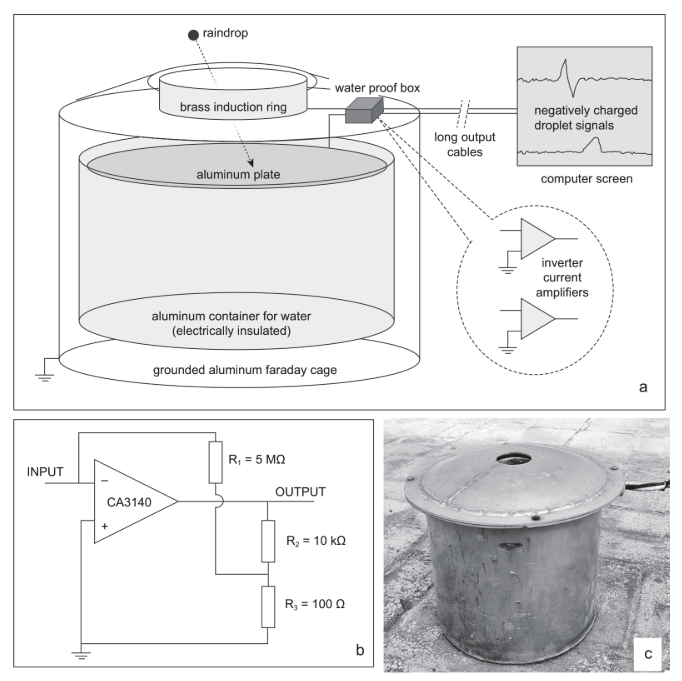
\includegraphics[width=0.7\textwidth]{figures/instrumento_de_medicion.png}
    \caption{(a) Diagrama del dispositivo de medición; (b) circuito amplificador inversor de corriente; (c) fotografía del dispositivo en el techo de la Facultad de Matemática, Astronomía, Física y Computación, Universidad Nacional de Córdoba.}
    \label{fig:instrumento_medicion}
\end{figure}

La jaula de Faraday presenta una abertura ligeramente mayor que el anillo, permitiendo que las gotas de lluvia entren únicamente a través del anillo de inducción. Toda el agua que llega a la placa se drena a través de sus lados y se recolecta en un contenedor de aluminio, que también está situado dentro de la jaula de Faraday pero eléctricamente aislado de ella.

Las gotas cargadas eléctricamente inducen corrientes tanto en el anillo como en la placa. Al caer una gota, primero se acerca al anillo. Al hacerlo, se induce una corriente de la polaridad opuesta a la carga de la gota. Luego, al alejarse, esta polaridad se invierte. Mientras tanto, la gota se acerca a la placa, induciendo también una corriente de polaridad opuesta a la carga de la gota, lo cual culmina en una meseta en la corriente dado que la placa de aluminio absorbe el impacto de la gota y se le transfiere toda la carga a la placa, la cual se disipa en el tiempo. La figura \ref{fig:corriente_gotas} muestra la dinamica de la señal electrica registrada por los amplificadores.

\begin{figure}[H]
    \centering
    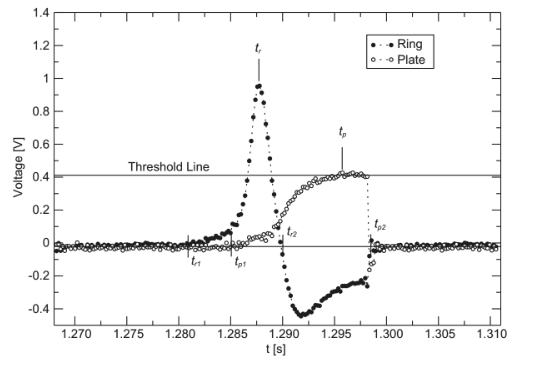
\includegraphics[width=0.7\textwidth]{figures/corriente_gotas.png}
    \caption{Corriente inducida por una gota cargada negativamente en el anillo (puntos solidos) y la placa (puntos huecos).}
    \label{fig:corriente_gotas}
\end{figure}

La recolección de datos se realiza a una tasa de 5 kHz por canal (5000 datos por segundo). Por limitaciones de hardware, no se puede realizar la recolección al mismo tiempo que la escritura a disco, por lo que cada segundo se pierden aproximadamente $50ms$ de datos, lo cual produce un "hueco" de datos en la señal.

\subsection{Procesamiento de Señales}
\lhead{}
\rhead{Procesamiento de Señales}

El procesamiento transforma las señales crudas registradas por el instrumento en una lista de propiedades fisicas para cada gota. Para ello se emplean dos programas que se ejecutan de manera secuencial: el primero realiza un preprocesamiento de las señales y el segundo extrae la información de las gotas y calcula sus características.

El fragmento de la señal que forma parte de una gota extraida por el programa, la denominamos `pulso'. Estos pulsos son reconocibles en la señal gracias a la dinamica producida por la interaccion de la gota con el instrumento de medicion.

El flujo general consta de cinco pasos principales:

\begin{enumerate}
    \item Rellenado de huecos en los datos.
    \item Remoción del offset de las señales.
    \item Búsqueda de pulsos en las señales.
    \item Aplicación de filtros de calidad para extraer los pulsos.
    \item Cálculo de propiedades de los pulsos.
\end{enumerate}

Para el procesamiento de los datos se han desarrollado dos programas en Fortran que trabajan de manera secuencial.

El primer programa se encarga del preprocesamiento de los datos, específicamente del rellenado de huecos mediante interpolación lineal y de la remoción del offset de las señales.

El segundo programa realiza el análisis principal de las señales ya preprocesadas. Implementa el algoritmo de detección de pulsos, aplica filtros para separar los pulsos válidos y calcula sus propiedades físicas, incluyendo carga eléctrica, velocidad de caída y tamaño.

\subsection{Necesidad de Mejoras}
\lhead{}
\rhead{Necesidad de Mejoras}

El código actual, aunque funcional, presenta varios problemas tanto en su diseño como en su rendimiento.

En primer lugar, el código consta de pocos archivos con una gran cantidad de líneas, lo que dificulta su mantenimiento y modificación. Cualquier cambio requiere revisar y entender todo el código, ya que las responsabilidades no están bien asignadas. Además, hay muchas variables sin nombres descriptivos y constantes hard-codeadas sin referencia alguna, lo que complica aún más la comprensión.

En segundo lugar, para grandes volúmenes de datos, la ejecución es muy lenta. Por ejemplo, para procesar datos de una tormenta de 5 horas de duración (aproximadamente 100 millones de datos), el programa tarda alrededor de 6 horas en completarse. A esto se suma un consumo de memoria excesivamente alto, lo que obliga a procesar los datos de a partes. A su vez el algoritmo actual no tiene en cuenta los pulsos que quedan en medio de estos cortes, resultando en la pérdida de algunos datos.

\subsection{Objetivos}
\lhead{}
\rhead{Objetivos}

\subsubsection{Objetivo General}

Desarrollar un sistema modular y automatizado para el análisis de datos de gotas cargadas eléctricamente que mejore significativamente la eficiencia, mantenibilidad y escalabilidad del código existente, facilitando la obtención de nuevos resultados.

El nuevo sistema debe ser capaz de procesar grandes volúmenes de datos de manera eficiente y, como mínimo, detectar la misma cantidad de pulsos que el código original, intentando incrementarla en lo posible.

\subsubsection{Objetivos Específicos}

\begin{enumerate}
    \item \textbf{Diseñar una arquitectura modular} que separe las etapas del procesamiento en al menos tres componentes independientes y reutilizables.

    \item \textbf{Optimizar el rendimiento y el uso de memoria} del algoritmo de detección de pulsos para manejar aproximadamente 100 millones de muestras (que corresponden a una tormenta de 5 horas de duración) utilizando menos de 2 GB de memoria y reduciendo el tiempo de análisis de 6 horas a aproximadamente 15 minutos, asegurando al menos la misma cantidad de pulsos detectados que el programa original.

    \item \textbf{Desarrollar un sistema de automatización} que permita ejecutar la cadena completa de análisis con un único comando y sin intervención manual.

    \item \textbf{Documentar completamente} el sistema mediante un manual de usuario y comentarios en el código para facilitar su uso y mantenimiento futuro.
\end{enumerate}

\subsection{Estructura de la Tesis}
\lhead{}
\rhead{Estructura de la Tesis}

La estructura de esta tesis está organizada de manera que primero se establece el contexto y la motivación del trabajo, luego se presenta el análisis del sistema existente, y finalmente se describe la solución propuesta y sus resultados. El documento se divide en las siguientes secciones:

\begin{enumerate}
    \item Presenta los conceptos previos necesarios, incluyendo una introducción al análisis de complejidad computacional que fundamenta las optimizaciones posteriores. (Sección 2)

    \item Realiza un análisis exhaustivo del código existente, describiendo los algoritmos actuales, identificando problemas de diseño y rendimiento, y motivando la necesidad de refactorización. (Sección 3)

    \item Presenta los algoritmos optimizados y estructuras de datos eficientes utilizados en el nuevo sistema. (Sección 4)

    \item Describe el nuevo algoritmo de deteccion de pulsos implementado. (Sección 5)

    \item Presenta el sistema de automatización desarrollado en Python. (Sección 6)

    \item Muestra los resultados obtenidos, incluyendo comparativas de rendimiento y precisión, seguida de las conclusiones y limitaciones del trabajo. (Sección 7)
\end{enumerate}

\section{Conceptos previos}

\subsection{Análisis de complejidad computacional}
\lhead{}
\rhead{Análisis de Complejidad Computacional}

Para evaluar y comparar la eficiencia de los algoritmos utilizados en este trabajo, es fundamental entender cómo se mide el rendimiento computacional. La notación Big-O es una herramienta matemática que permite describir el comportamiento asintótico de un algoritmo en términos de tiempo de ejecución o uso de memoria, en función del tamaño de la entrada.

\subsubsection{Notación Big-O}

La notación Big-O describe el límite superior del crecimiento de una función. Formalmente, decimos que $f(n) = O(g(n))$ si existen constantes positivas $c$ y $n_0$ tales que $f(n) \leq c \cdot g(n)$ para todo $n \geq n_0$.

En el contexto de algoritmos, esto significa que el tiempo de ejecución o el uso de memoria no crecerá más rápido que la función $g(n)$ multiplicada por una constante, independientemente del tamaño de la entrada.

\subsubsection{Clases de complejidad comunes}

Las clases de complejidad más relevantes para este trabajo son:

\begin{itemize}
    \item \textbf{$O(1)$ - Constante:} El tiempo de ejecución es independiente del tamaño de la entrada. Ejemplo: acceder a un elemento de un arreglo por índice.
    
    \item \textbf{$O(\log n)$ - Logarítmica:} El tiempo crece logarítmicamente con el tamaño de la entrada. Ejemplo: búsqueda binaria en un arreglo ordenado.
    
    \item \textbf{$O(n)$ - Lineal:} El tiempo es proporcional al tamaño de la entrada. Ejemplo: recorrer todos los elementos de un arreglo.
    
    \item \textbf{$O(n \log n)$ - Lineal logarítmica:} El tiempo crece como $n$ multiplicado por $\log n$. Ejemplo: algoritmos de ordenamiento eficientes como merge sort.
    
    \item \textbf{$O(n^2)$ - Cuadrática:} El tiempo es proporcional al cuadrado del tamaño de la entrada. Ejemplo: algoritmos de ordenamiento simples como bubble sort.
\end{itemize}

En la figura \ref{fig:complejidades_algoritmicas} se puede observar un gráfico comparativo de numero de operaciones vs tamaño de datos para diferentes complejidades algorítmicas

\begin{figure}[H]
    \centering
    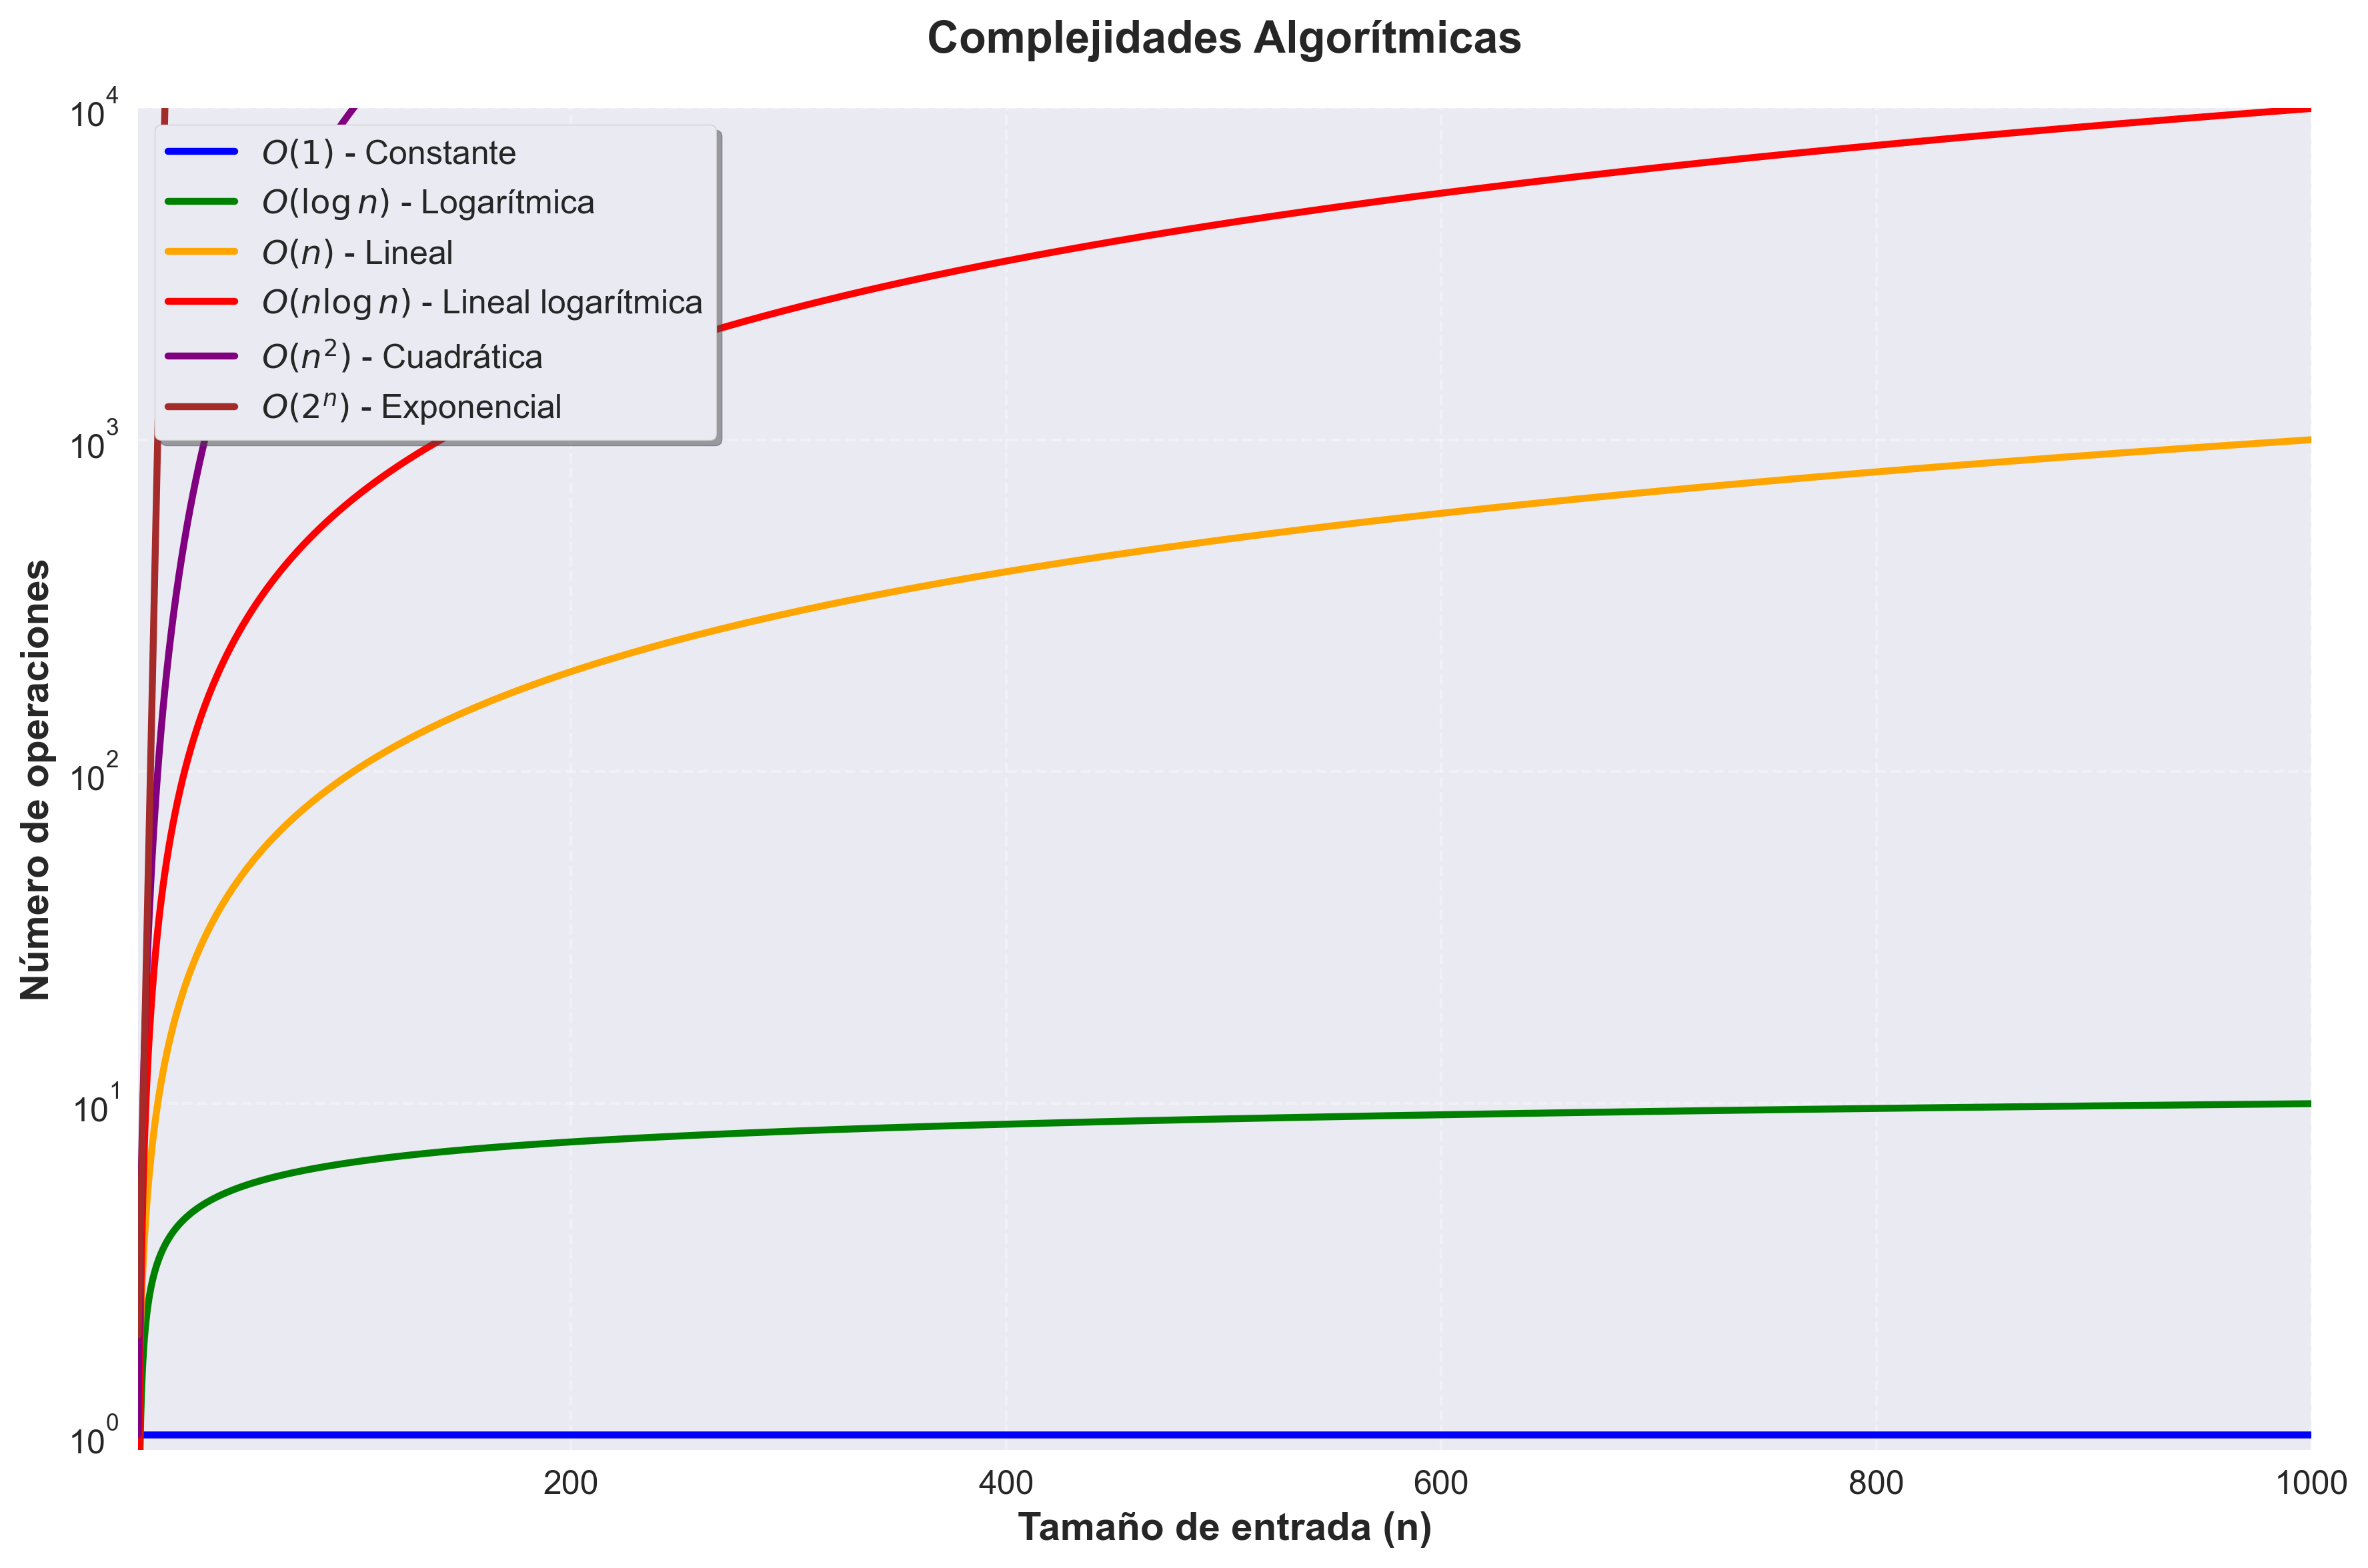
\includegraphics[width=0.8\textwidth]{figures/complejidades_algoritmicas.png}
    \caption{Gráfico comparativo de numero de operaciones vs tamaño de datos para diferentes complejidades algorítmicas, en escala logarítmica. }
    \label{fig:complejidades_algoritmicas}
\end{figure}

\subsubsection{Importancia en el contexto de este trabajo}

En el procesamiento de señales, donde se manejan millones de puntos de datos, la diferencia entre algoritmos de complejidad $O(n)$ y $O(n^2)$ puede resultar en diferencias de horas en el tiempo de procesamiento. Por ejemplo, para procesar 100 millones de puntos:

\begin{itemize}
    \item Un algoritmo $O(n)$ podría completarse en segundos
    \item Un algoritmo $O(n^2)$ podría requerir días o semanas
\end{itemize}

Por esta razón, la optimización de la complejidad computacional es crucial para hacer viable el análisis de grandes volúmenes de datos meteorológicos en tiempo razonable.

\section{Análisis del código existente}
\lhead{}
\rhead{Análisis del código existente}

Antes de comenzar a desarrollar el nuevo sistema, fue fundamental analizar el código existente. El programa consta de dos archivos Fortran (`promedio\_general.f' y `buscador\_de\_gotas.f') donde toda la lógica está implementada directamente en el entorno global del programa, sin modularización alguna. 

\subsection{Descripción del algoritmo actual}
A continuación se describe el funcionamiento de los dos programas que conforman el sistema actual.

\subsubsection{Programa de preprocesamiento}

El primer programa (`promedio\_general.f') recibe como entrada las señales crudas registradas por el instrumento y realiza dos operaciones fundamentales:    

\begin{enumerate}


\item \textbf{Lectura de datos:} El programa lee los archivos de datos crudos y los convierte en señales. El formato de los archivos es un archivo `.lvm' que contiene 3 columnas: tiempo, señal del anillo y señal de la placa.

\item \textbf{Rellenado de huecos mediante interpolación:} Debido a las limitaciones de
hardware mencionadas anteriormente, cada segundo se pierden aproximadamente
$50ms$ de datos durante la adquisición. El programa identifica estos huecos y los
rellena utilizando interpolación lineal el punto anterior y el posterior al hueco.

\item \textbf{Remoción del offset de las señales:} Para cada punto de la señal, se calcula el
promedio de los 5000 puntos circundantes (2500 puntos a cada lado) y se le resta este
valor. Para esto se ignoran los primeros y últimos 2500 puntos de la señal.

Este proceso elimina el offset de corriente continua que puede variar durante la medición.

\item \textbf{Salida de resultados:} Finalmente, se escriben las señales preprocesadas en un archivo. El formato de salida son 4 columnas: contador de tiempo (entero), señal del anillo resultante, señal de la placa resultante y un booleano que indica si la fila corresponde a un hueco.

\end{enumerate}

\subsubsection{Programa de detección de pulsos}

El segundo programa (`buscador\_de\_gotas.f') implementa el algoritmo principal de
detección y análisis. El flujo general consta de las siguientes etapas:

\begin{enumerate}

\item \textbf{Lectura y preprocesamiento de datos:} El programa lee los archivos de datos
preprocesados con el paso anterior. Se pueden leer hasta 36 archivos, y cada archivo puede contener hasta 13 millones de muestras.

\item \textbf{Detección de pulsos mediante umbrales:} Se implementa un sistema de umbrales que varía dinámicamente desde un valor superior (`2.00') hasta
uno inferior (`0.02') a lo largo de 1000 pasos. Esta variación permite
detectar pulsos de diferentes amplitudes.
Para cada umbral, se buscan pares de puntos consecutivos que superen el umbral en ambas señales (anillo y placa), con una separación máxima de 100 puntos. Al primer punto del par consecutivo en cada señal, se lo denomina `c1' y `c2' respectivamente. En la figura \ref{fig:sensores_gota} se puede observar un pulso de ejemplo detectado con este algoritmo.

\begin{figure}[H]
    \centering
    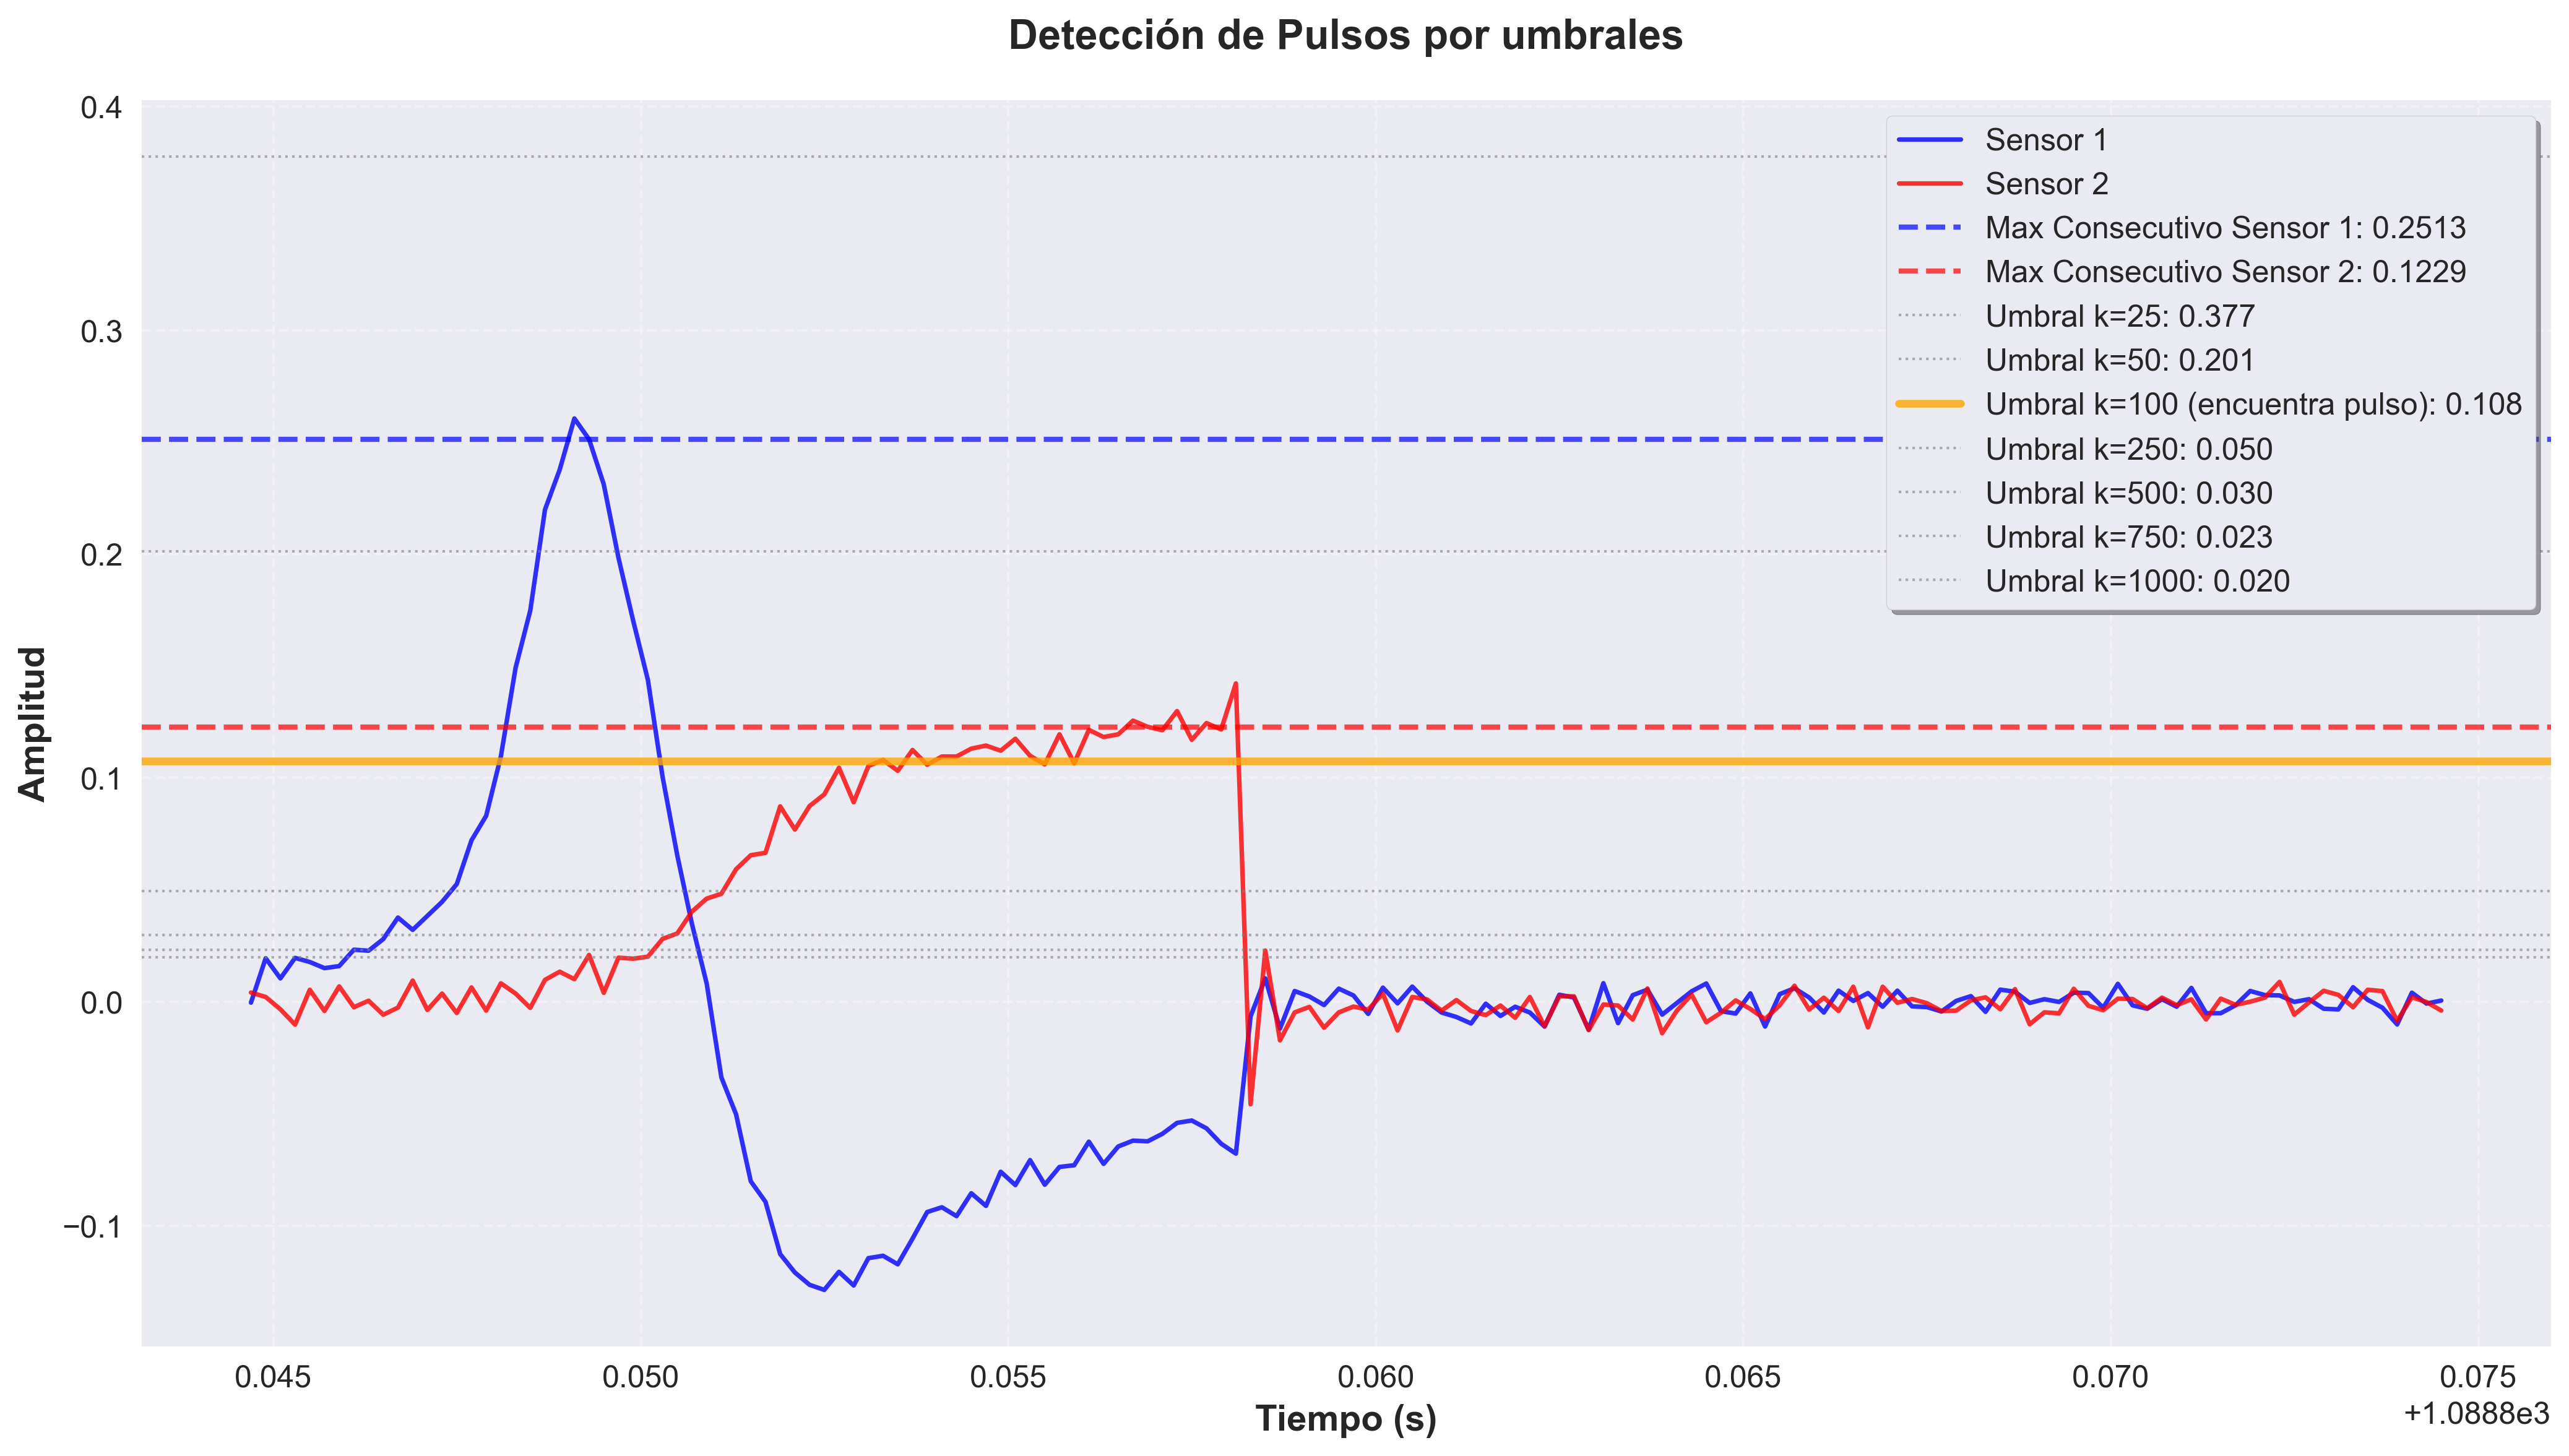
\includegraphics[width=0.9\textwidth]{figures/sensores_gota.png}
    \caption{En la figura se puede observar un pulso, junto con los maximos consecutivos de cada sensor. Ademas se observan distintos valores de umbrales, y se marca el umbral que encuentra el pulso. }
    \label{fig:sensores_gota}
\end{figure}

\item \textbf{Localización y delimitación de pulsos:} Una vez detectado un pulso, se determina el "inicio" de cada señal (u1 y u2 respectivamente), retrocediendo desde c1 y c2 respectivamente hasta encontrar el punto donde la señal se anula.
Se calcula tambien el punto medio de la señal del anillo (p1) avanzando desde c1 hasta donde se anula la señal, y el punto de quiebre de la señal de la placa (p2) mediante análisis de la integral de la misma. En la figura \ref{fig:analisis_gota} se pueden observar estos puntos relevantes.
El algoritmo recorta cada pulso en base a la localización de estos puntos, considerando un ancho máximo de 400 puntos.

\begin{figure}[H]
    \centering
    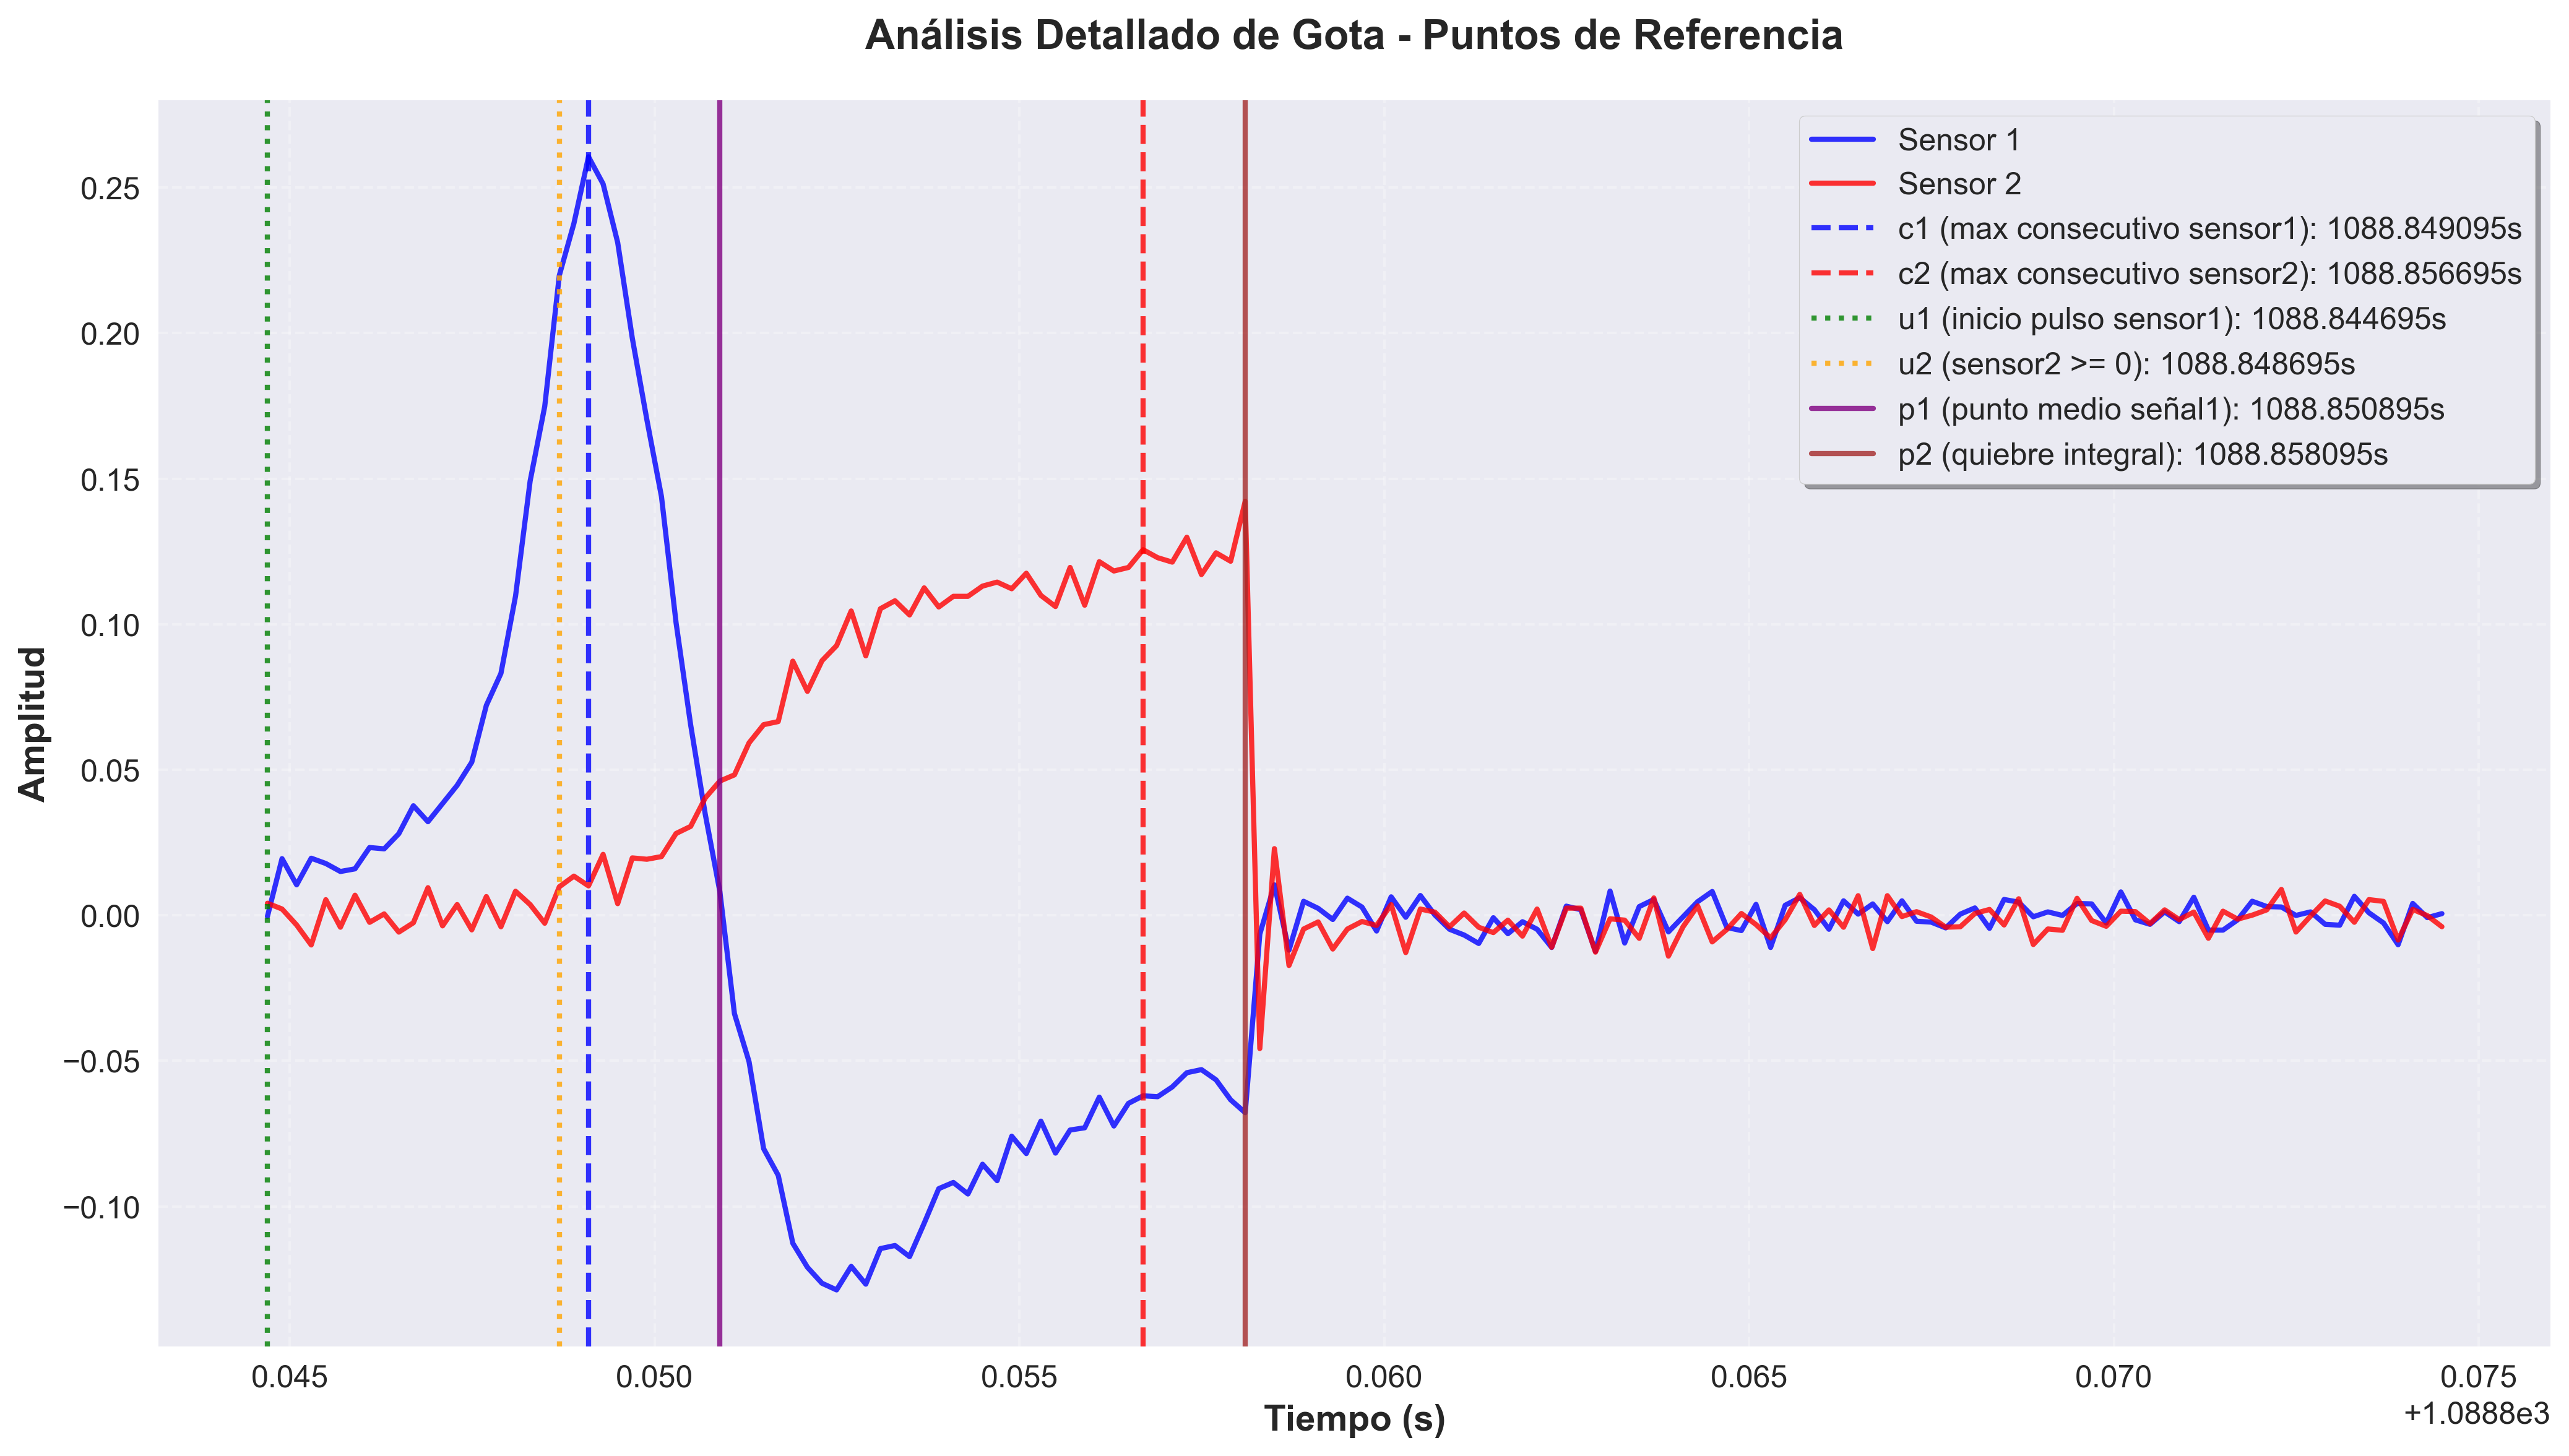
\includegraphics[width=0.9\textwidth]{figures/analisis_gota.png}
    \caption{La figura muestra un pulso detectado junto con sus puntos relevantes.}
    \label{fig:analisis_gota}
\end{figure}


\item \textbf{Cálculo de propiedades físicas:} Para cada pulso detectado, se calculan:

\begin{itemize}
    \item Carga eléctrica: Se integra la señal de ambos canales y se aplica el factor de
    conversión correspondiente a la amplificación del instrumento. La integración de la señal se fundamenta en el principio físico de que la carga eléctrica inducida en un conductor es proporcional a la integral temporal de la corriente que fluye a través de él. En la figura \ref{fig:calculo_carga_electrica} se puede observar el cálculo de carga eléctrica mediante integración de señales del anillo y placa.
    \item Velocidad de caída: Se determina mediante la separación conocida entre
    anillo y placa (5.7 cm) dividida por el tiempo que hay entre el punto medio de la señal del anillo y el punto de quiebre de la señal de la placa.
    \item Diámetro: Se obtiene interpolando en una tabla velocidad-diámetro precalculada. En la figura \ref{fig:relacion_velocidad_diametro} se puede observar la relación velocidad-diámetro para gotas de lluvia.
\end{itemize}

\begin{figure}[H]
    \centering
    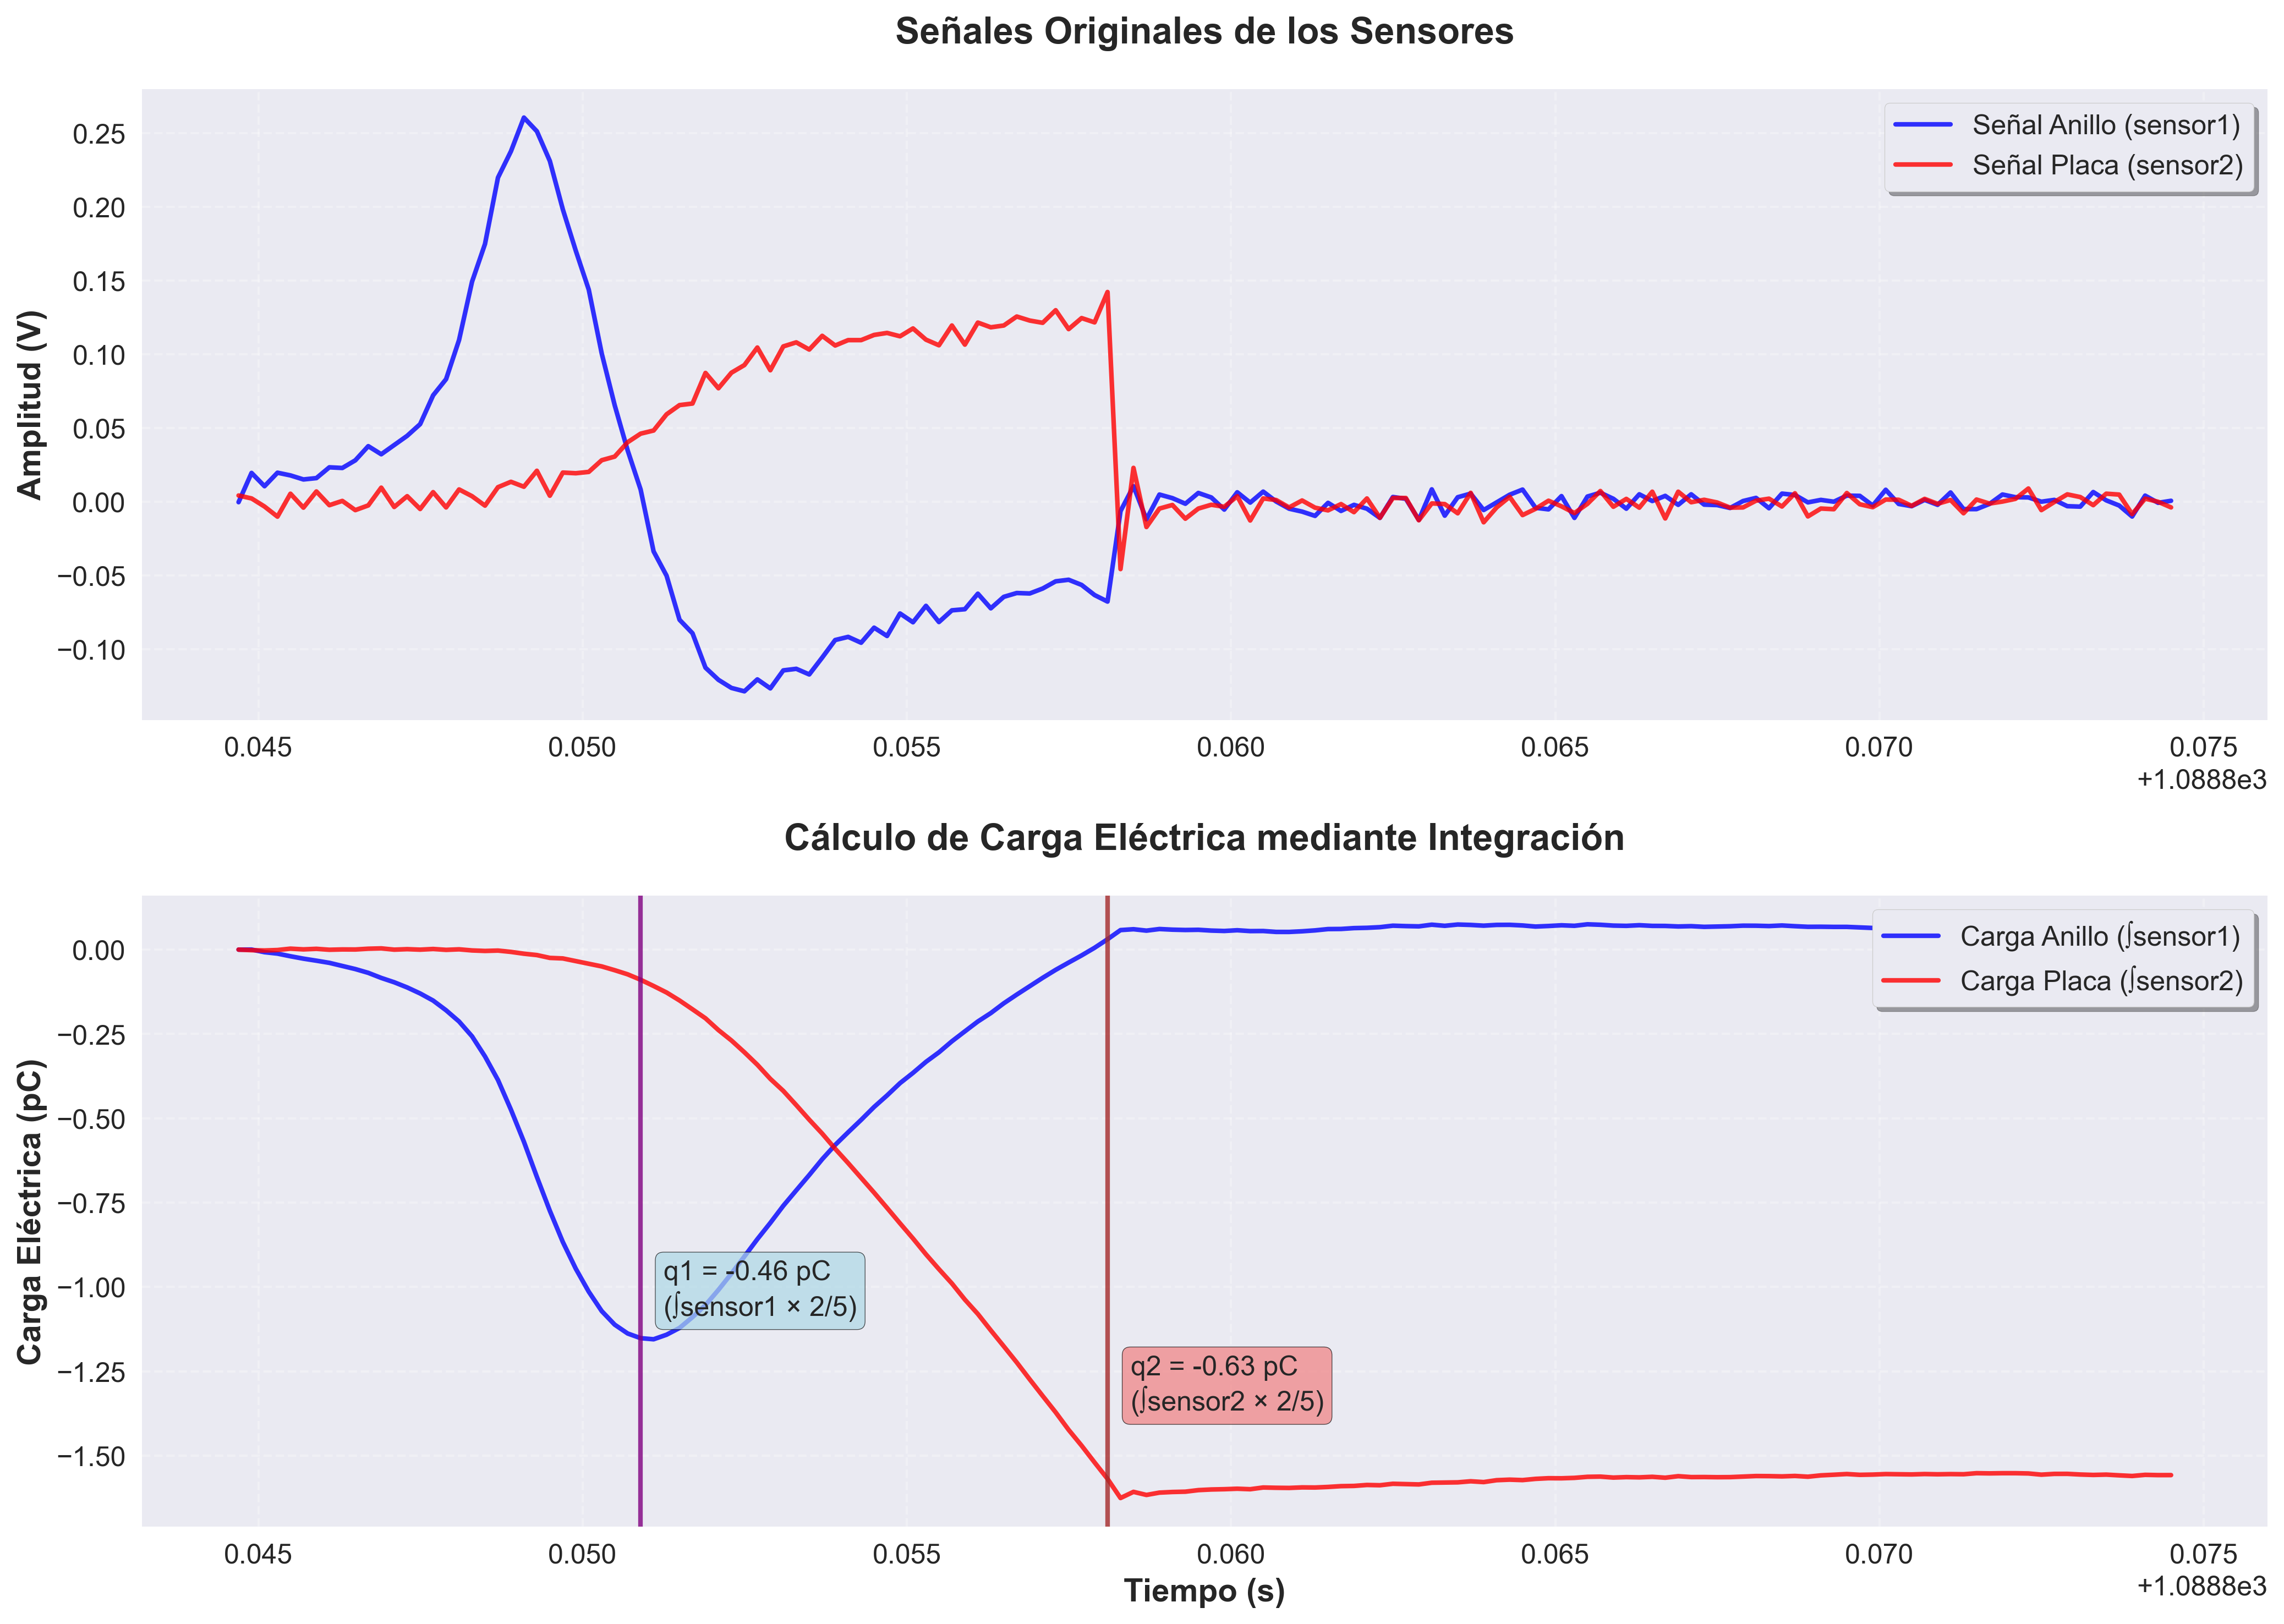
\includegraphics[width=0.9\textwidth]{figures/calculo_carga_electrica.png}
    \caption{Cálculo de carga eléctrica mediante integración de señales del anillo y placa. Se debe tener en cuenta que la integral es de signo opuesto ya que la señal es inversora.}
    \label{fig:calculo_carga_electrica}
\end{figure}

\begin{figure}[H]
    \centering
    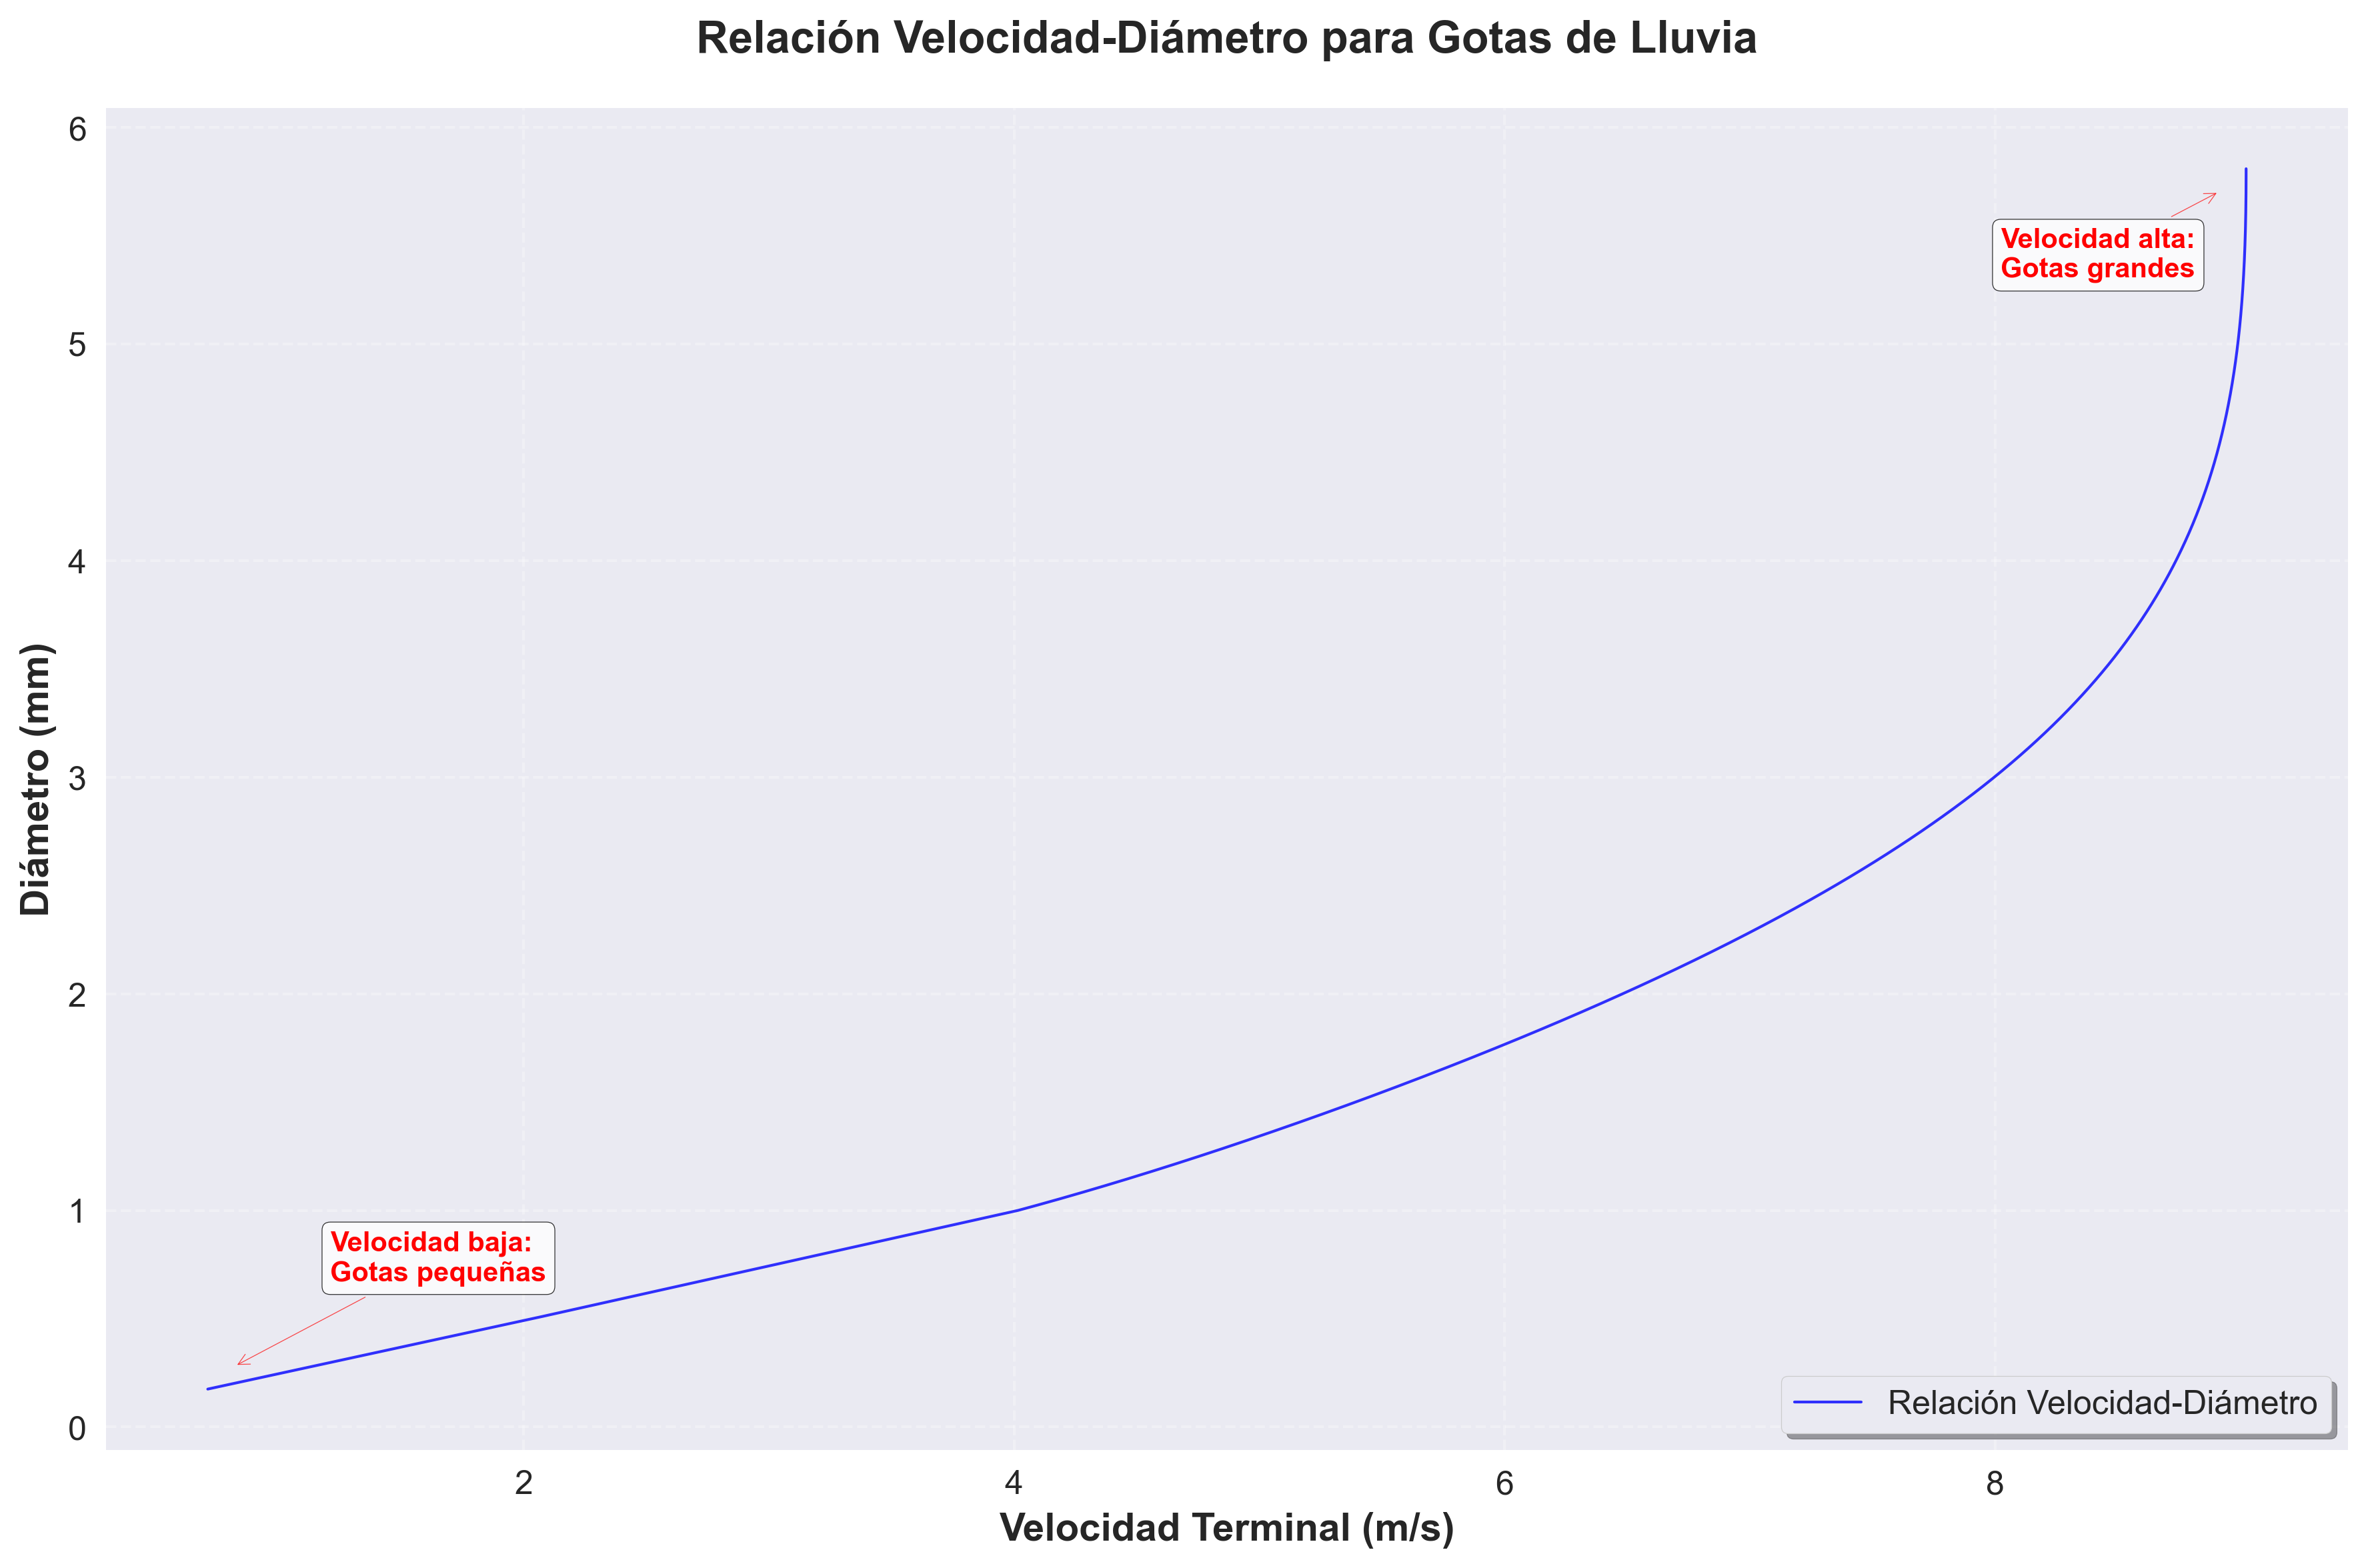
\includegraphics[width=0.9\textwidth]{figures/relacion_velocidad_diametro.png}
    \caption{Relación velocidad-diámetro para gotas de lluvia.}
    \label{fig:relacion_velocidad_diametro}
\end{figure}


\item \textbf{Aplicación de filtros de calidad:} Durante el proceso de detección, el algoritmo identifica tanto pulsos validos (que corresponden a gotas de lluvia reales), asi como falsos positivos claros (que corresponden a ruido o detecciones espurias)

Para resolver este problema, se implementan filtros de calidad para separar los pulsos válidos de los que no lo son. Estos filtros eliminan detecciones que no cumplen con propiedades fisicas esperadas para gotas de lluvia reales. Los filtros se aplican de manera progresiva, donde cada etapa elimina un tipo específico de detección errónea:

\begin{itemize}

\item \textbf{Filtros de carga:} La carga de la gota tanto en el anillo como en la placa tiene
que ser mayor a un valor mínimo (`qminima=0.2') (en valor absoluto).

\item \textbf{Filtro de signo:} Se verifica que la carga del pulso sea del mismo signo en
ambos canales.

\item \textbf{Filtro de velocidad:} Se verifica que la distancia temporal entre los picos del
anillo y la placa corresponda a una velocidad de caída físicamente plausible
(entre 0.7125 y 11.4 m/s).

\end{itemize}

\item \textbf{Sistema de evaluación y ordenamiento:} Una vez aplicados los filtros de calidad, las detecciones restantes corresponden principalmente a gotas. Algunas de estas presentan señales muy limpias y bien definidas, mientras que otras pueden tener pequeñas distorsiones, ruido residual, o características que sugieren mediciones menos precisas.

Para clasificar las gotas obtenidas, se implementa un sistema de puntuación que evalúa la calidad de cada detección mediante cinco criterios independientes. Este sistema fue desarrollado mediante ajuste manual y experimental, donde se analizaron visualmente detecciones para identificar patrones que distinguían entre gotas de alta y baja calidad.

\begin{itemize}

    \item \textbf{Eval1 y Eval2:} Diferencia cuadrática entre la integral de la señal real y dos modelos teóricos distintos
    del pulso.
    Para el pulso del anillo se utiliza el siguiente modelo:
    
    \begin{equation}
        a_1(t) = \frac{30.6 \cdot q_1}{\left(30.6^{1/1.7} + \left(\frac{v}{50.7}\right)^2(t-p_1)^2\right)^{1.7}}
    \end{equation}
    
    Para el pulso de la placa se utiliza un modelo por partes:

    \begin{equation}
        a_2(t) = \begin{cases}
            0 & \text{si } t < u_2 \\
            q_2 \cdot \left(\frac{t-u_2}{p_2-u_2}\right)^{1.373} & \text{si } u_2 \leq t < p_2 \\
            q_2 & \text{si } t \geq p_2
        \end{cases}
    \end{equation}

    donde $q_1$ y $q_2$ son las cargas medidas en el anillo y la placa respectivamente, $v$ es la velocidad de la gota, $p_1$ es el punto medio del pulso del anillo, $p_2$ es el punto de quiebre de la integral del pulso de la placa, y $u_2$ es el punto inicial del pulso de la placa.

    En la figura \ref{fig:comparacion_modelos_teoricos} se puede observar la comparación entre señales reales y modelos teóricos para pulsos del anillo y placa.

    \begin{figure}[H]
        \centering
        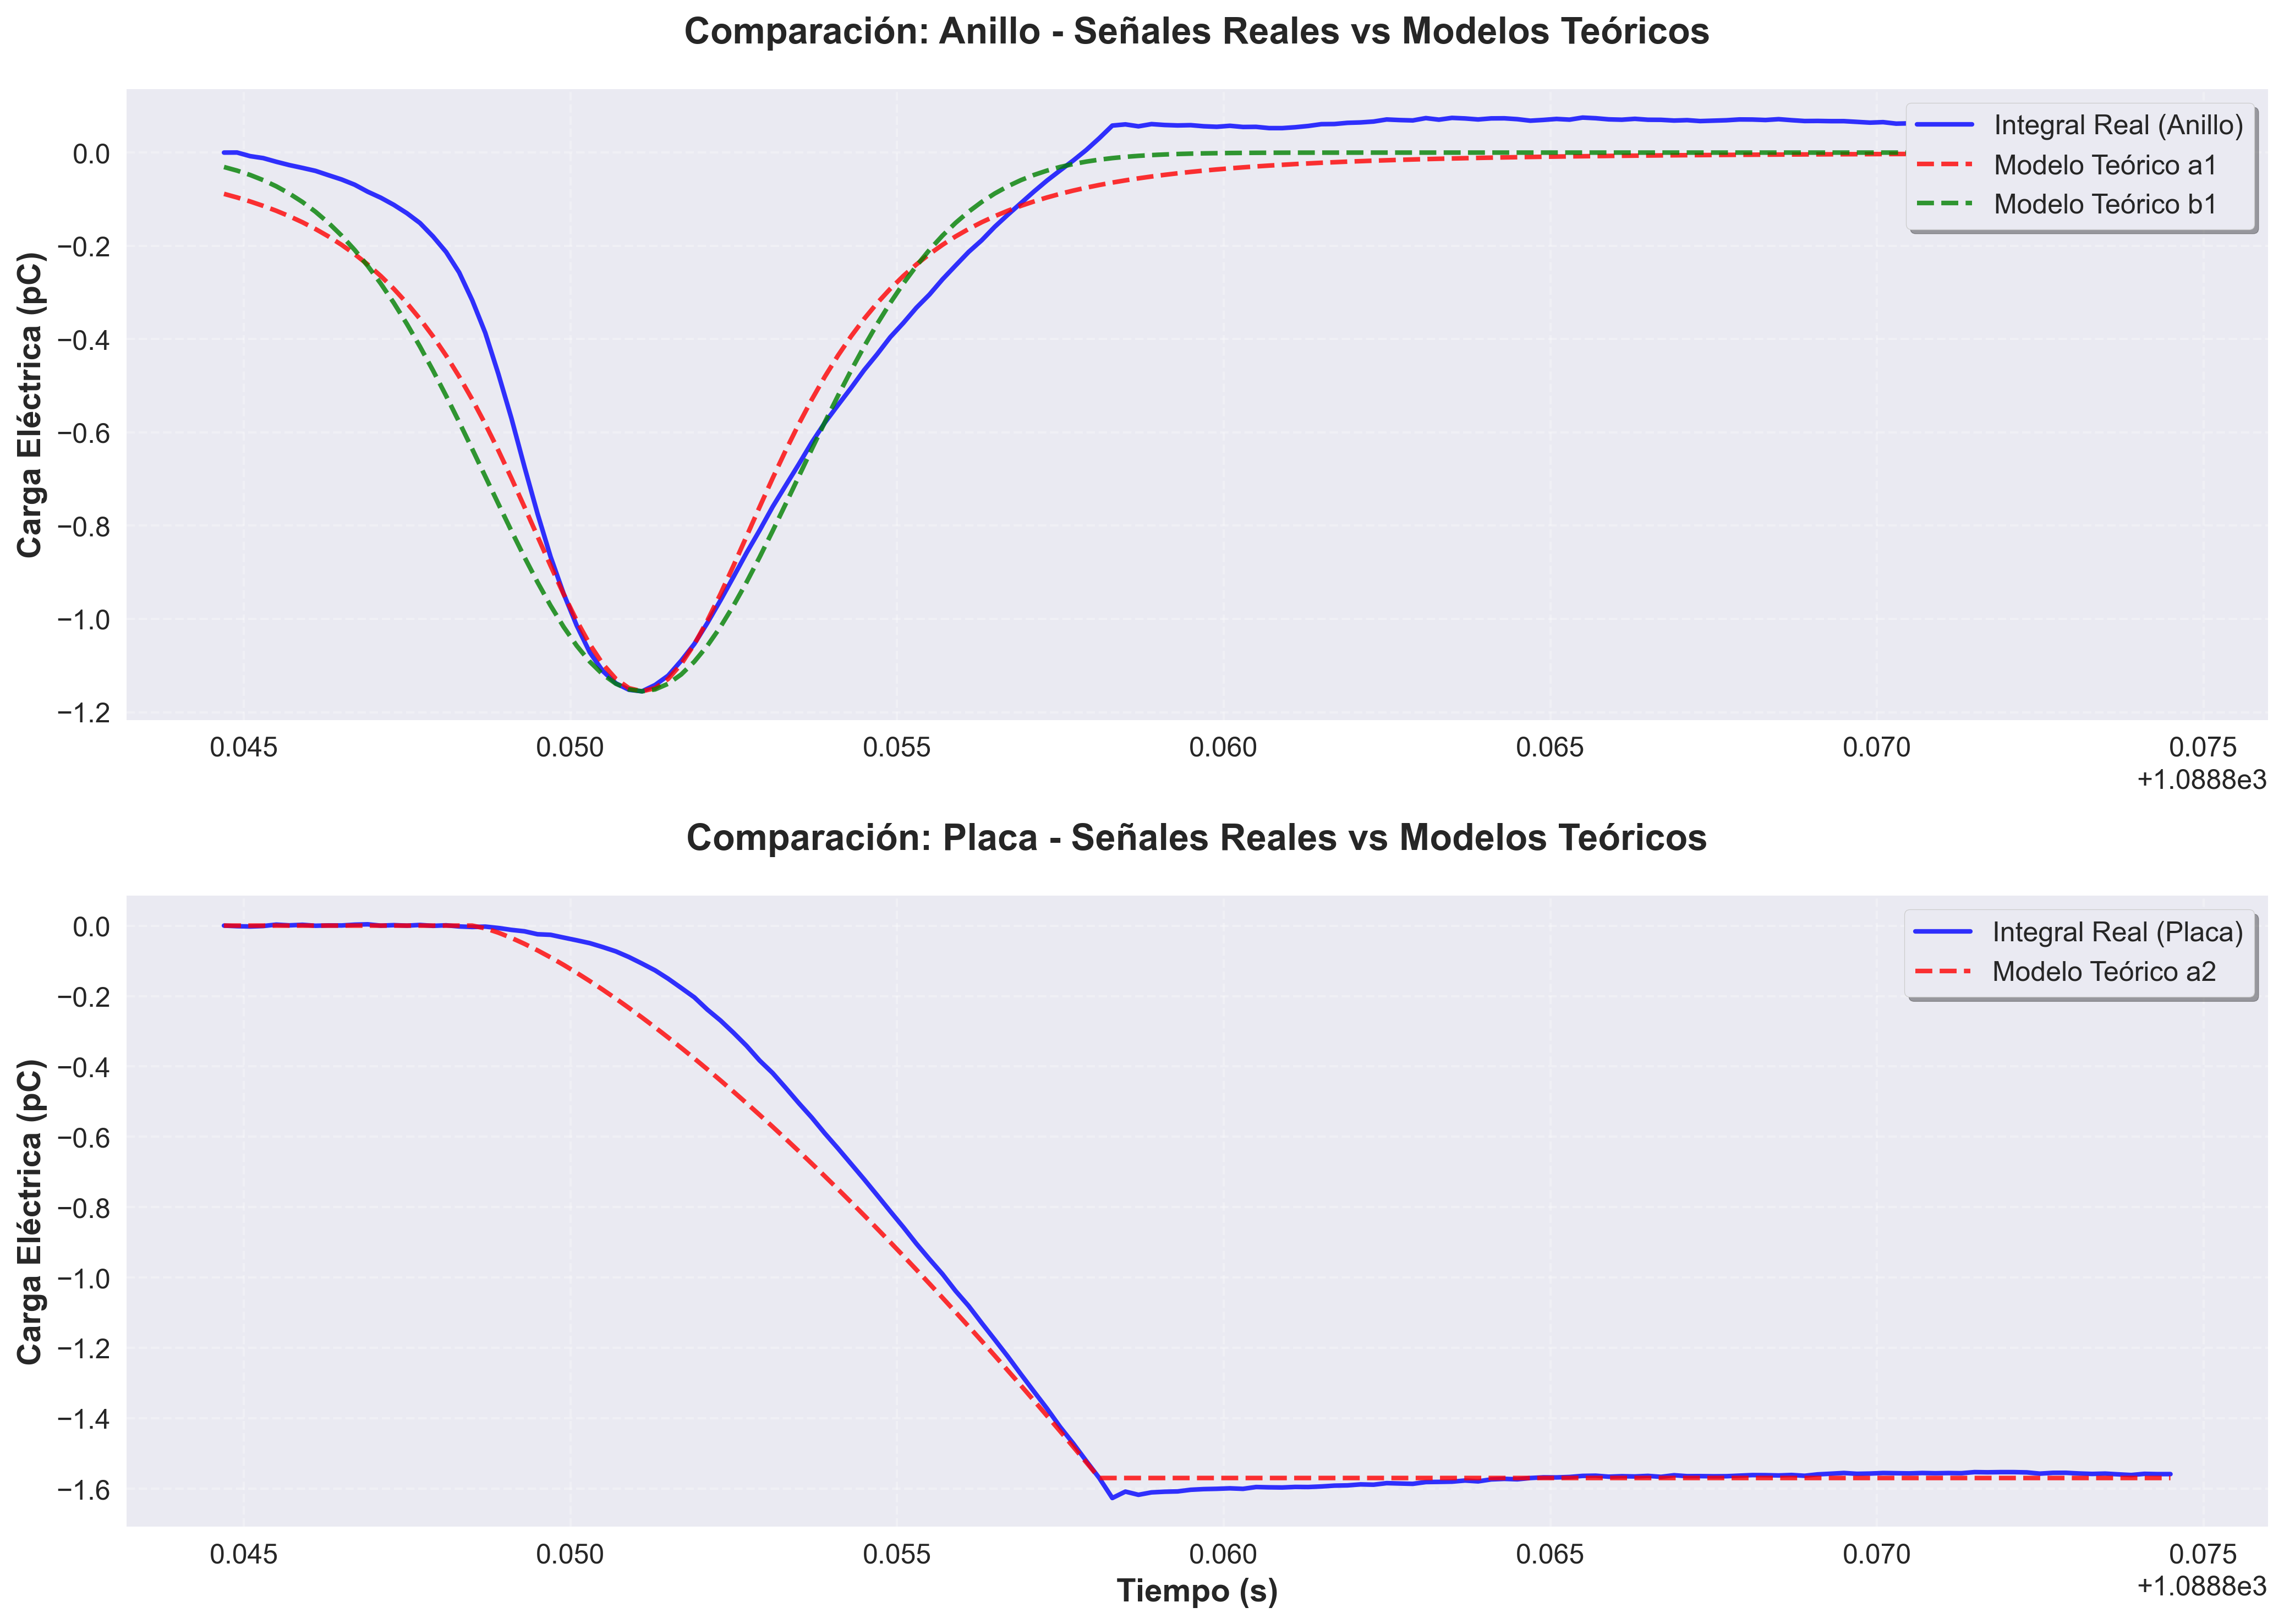
\includegraphics[width=0.9\textwidth]{figures/comparacion_modelos_teoricos.png}
        \caption{Comparación entre señales reales (integrales) y modelos teóricos para pulsos del anillo y placa.}
        \label{fig:comparacion_modelos_teoricos}
    \end{figure}

    \item \textbf{Eval3:} Desviación de la proporción esperada entre cargas del anillo y la placa. Experimentalmente se observo que la carga medida en el anillo es aproximadamente el 87\% de la carga medida en la placa, por lo que se mide la desviacion de esta proporcion.

    \begin{equation}
        penal2(l) = \left|\frac{q_1}{q} - 0.87 \cdot \frac{q_2}{q}\right|
    \end{equation}

    donde $q$ esta definido como $q = \frac{q1 / 0.87 + q2}{2}$
    
    \item \textbf{Eval4:} Desviación de la proporción esperada del ancho entre los picos de la
señal de la placa y el anillo. Experimentalmente se observo que el ancho del pulso de la placa es aproximadamente el 79\% del ancho del pulso del anillo, por lo que se mide la desviacion de esta proporcion.

    \begin{equation}
        penal3(l) = \left|\frac{p_1}{p} - 0.79 * \frac{p_2}{p}\right|
    \end{equation}

    donde $p$ esta definido como $p = \frac{p_1 / 0.79 + p_2}{2}$

    \item \textbf{Eval5:} Proporción de señal en el rango de ruido (entre -0.02 y 0.02). Para esto se computan los promedios de cada señal, y se cuentan los puntos que, cuando se les resta el promedio, estan entre -0.02 y 0.02.

\end{itemize}

    Las evaluaciones se combinan linealmente con pesos para finalmente obtener una puntuacion total, que esta en el range $[0, 20]$. Mientras mas chico sea el valor de la puntuacion total, mejor es la calidad de la gota.
    
\item \textbf{Salida de resultados:} Finalmente, se escriben los datos de todos los pulsos válidos
en un archivo, incluyendo posición temporal, cargas, velocidad, diámetro y puntuación de calidad.

\end{enumerate}

\subsection{Problemas de diseño}

El código existente presenta problemas de diseño que dificultan su comprensión y mantenimiento:

\begin{itemize}

\item \textbf{Modularización inexistente:} Todo el procesamiento está en el entorno global del programa, que maneja todos los pasos de procesamiento, como la detección de pulsos, cálculo de características, aplicación de filtros, escritura de resultados, etc. Cualquier modificación requiere entender por completo como interactuan las diferentes `partes' del programa.

\item \textbf{Variables sin contexto semántico:} El código utiliza variables como `s', `ss', `i', `j', `w', `k', `l', `p', `r', `x', `cont', `contt', `cc1', `cc2', `iii' sin ningún contexto. Es
imposible determinar qué representa cada una sin leer todo el código. Ademas, estan todas definidas en el principio del programa, lo cual hace que sea dificil entender su uso en el resto del código.
    
\item \textbf{Requiere dividir el conjunto de datos en varias partes}: El consumo de memoria es muy alto, por lo que el programa requiere dividir el conjunto de datos en varias partes y procesarlos secuencialmente. Esto hace que se pierdan algunos pulsos, ya que los que quedan en medio de los cortes no se procesan.

\item \textbf{Lectura de archivos hard-codeada:} El programa requiere cambio en los nombres de los archivos a procesar, ya que los nombres de estos son constantes en el codigo en vez de ser parametros. Ademas, hay un bloque de codigo que permite leer hasta 36 archivos, que se debe comentar o descomentar dependiendo de la cantidad en la que se dividio el conjunto de datos a procesar.

\item \textbf{Codigo duplicado:} La cantidad de codigo repetido es muy alta. Hay mucha logica la cual solo tiene un cambio en el signo, un cambio en un `if statement' o un cambio en una variable. Esto hace que sea dificil mantener el codigo ya que hay que modificarlo en varios lugares.

\end{itemize}

\subsection{Problemas de rendimiento}

Al analizar el rendimiento del código, se encontraron dos areas de potenciales mejoras:

\begin{itemize}
    \item \textbf{Remoción de offset:} El algoritmo de remoción de offset es muy ineficiente. Como se puede observar en la implementación \nameref{lst:codigo_remocion_offset}, para cada punto, se hace una suma de 5001 valores divididos por 5001,
    resultando en una complejidad $$O(5001n) = O(n)$$ Obviamente se trata de una complejidad lineal, pero no solo que la constante es altisima por el factor de 5001, sino que tambien se realizan 5001 divisiones por cada punto, que no es la operacion mas eficiente en un procesador.

    \begin{lstlisting}[language=Fortran, label=lst:codigo_remocion_offset, caption={buscador\_de\_gotas.f - Algoritmo ineficiente de remoción de offset}]
! n = 5000
! ww es la cantidad de puntos en la señal
! w1 y w2 son los arreglos de las señales
        do j=1,ww
            if ((j.ge.n/2+1).and.(j.le.ww-n/2)) then
                do k=-n/2,n/2
                       w1p(j)=w1p(j)+w1(j+k)/(n+1)
                       w2p(j)=w2p(j)+w2(j+k)/(n+1)            
                enddo
                w1a(j)=w1(j)-w1p(j)
                w2a(j)=w2(j)-w2p(j)
            else 
                ind(j)=0
                w1a(j)=0
                w2a(j)=0
            endif	
            write(30,*) j,w1a(j),w2a(j),ind(j)
        enddo
    \end{lstlisting}


    \item \textbf{Detección de pulsos:} Si analizamos la complejidad de la implentacion de este algoritmo, podemos ver que para cada umbral (1000 umbrales), se revisa todo el array de la señales. Si dos puntos consecutivos superan el umbral en la primera señal, se revisa hasta un total de 100 puntos en la segunda señal. Esto resulta en una complejidad $$O(\#umbrales * \#puntos * 100) = O(100000 * \#puntos) = O(\#puntos)$$ Identico al caso anterior, se trata de una complejidad lineal, pero con una constante extremadamente alta.
\end{itemize}

\subsection{Motivación de la refactorización}

Todas las problematicas mencionadas anteriormente, motivan a realizar una refactorizacion del codigo. Esta refactorizacion tiene muchos beneficios, entre los cuales:

\begin{itemize}

\item \textbf{Mantenibilidad:} Cualquier corrección de errores o implementación de mejoras requiere revisar y entender menos codigo, ya que la logica se encuentra en funciones mas pequeñas.

\item \textbf{Reutilizabilidad:} El codigo puede ser reutilizado para otros experimentos o instrumentos.

\item \textbf{Verificación:} Permitiria realizar pruebas unitarias de cada funcion y no de todo el programa completo.

\item \textbf{Colaboración:} Otros investigadores pueden entender y modificar el código sin
invertir tanta cantidad de tiempo y esfuerzo estudiándolo.

\end{itemize}

\subsection{Problemas descubiertos durante la refactorización}

El programa `promedio\_general.f', como se menciono anteriormente, se encarga tanto del rellenado de huecos como de la remocion del offset de las señales. Es en esta primera parte donde se descubrio un error en la implementacion.

Basicamente, primero el algoritmo llena los huecos con un valor constante `10', para luego buscar los bordes de estos huecos y completarlos con una interpolacion lineal. En los comentarios del codigo, se menciona que esta interpolacion lineal se hace entre los promedios de los 1000 puntos anteriores y posteriores al hueco. Sin embargo, en la implementacion, se utiliza los valores de los extremos del huecos.

El código \nameref{lst:codigo_error} muestra la implementación del algoritmo de rellenado de huecos. Como se puede observar, los comentarios indican que se debe usar el promedio de 1000 puntos, pero la implementación utiliza directamente los valores de los bordes (`a1', `a2', `b1', `b2').

Este error tiene un impacto significativo en los pasos posteriores del procesamiento, particularmente en la remoción del offset. Al rellenar los huecos utilizando una interpolación entre dos valores puntuales, en lugar de promedios de ventanas más amplias, se pueden introducir distorsiones importantes. Esto ocurre especialmente cuando los valores utilizados para la interpolación corresponden a puntos críticos que difieren considerablemente del promedio de la señal en ese momento.

\begin{lstlisting}[language=Fortran, label=lst:codigo_error, caption={promedio\_general.f - Error en implementación de rellenado de huecos}]
* Busca donde esta un punto que tiene valor de 10. y 
* va hacia atras para encontrar el primer que no es
* igual a 10.
* es decir es un borde izquierdo de un 'hueco'
* tambien va hacia adelante para encontrar el borde
* derecho del 'hueco'
* despues promedia los numeros de cada canal
* 100 puntos hacia atras
* y 1000 puntos hacia adelante 
* y a esos promedios los llama a1 y a2 para el 
* primer canal y
* b1 y b2 para el segundo canal
* Despues el valor w1(j) y w2(j) los revalua como
* siguiendo una recta 
* entre esos dos promedios.
* Tambien ingresa un indice que vale 1 cuando no hay
* blanco y un 0 cuando si lo hay.

      do j=1,ww
         if (w1(j).eq.10.) then
            ind(j)=0
            
            do i=1,ww
               if ((j-i.gt.0.).and.(w1(j-i).ne.10.)) then
		     a1=w1(j-i)
		     b1=w2(j-i)                  
                     k1=i
                  goto 20
               endif
            enddo
            
 20         do i=1,ww  
               if ((j+i.le.ww).and.(w1(j+i).ne.10.)) then
		     a2=w1(j+i)
		     b2=w2(j+i)                  
                     k2=i-1
                  goto 30
               endif
            enddo

! Aca es donde se utiliza los valores de los extremos
! en vez de los promedios de 1000 puntos
 30         w1p(j)=(a2-a1)/real(k2+k1)*real(k1)+a1
            w2p(j)=(b2-b1)/real(k2+k1)*real(k1)+b1
         else
            ind(j)=1
            w1p(j)=w1(j)
            w2p(j)=w2(j)
         endif
      enddo
\end{lstlisting}

\section{Algoritmos y estructuras de datos utilizadas}
\lhead{}
\rhead{Algoritmos y estructuras de datos utilizadas}

Para abordar las limitaciones de performance del código existente, se utilizaron algoritmos y estructuras de datos eficientes que mantienen la misma o similar funcionalidad pero con un rendimiento superior.

\subsection{Optimización del algoritmo de promedio móvil}

El algoritmo de ventana deslizante (sliding window) es una técnica de optimización utilizada para resolver eficientemente problemas que involucran secuencias contiguas en arreglos. Es particularmente útil cuando se necesita mover una "ventana" de tamaño fijo o dinámico a través de los datos para realizar cálculos o encontrar patrones.

En nuestro caso, el problema de calcular el promedio móvil para remover el offset se ajusta perfectamente a esta técnica: necesitamos mantener una ventana de tamaño fijo que se mueve a través de la señal, calculando el promedio en cada punto. En lugar de recalcular la suma completa cada vez que la ventana se mueve (lo que requeriría sumar todos los elementos nuevamente), podemos mantener una suma acumulada que actualizamos incrementalmente.

Si analizamos la implementación \nameref{lst:codigo_promedio_movil}, vemos que el array de datos se recorre una sola vez. En cada iteración, solo se realiza una suma para agregar el nuevo valor a la ventana y una resta para eliminar el valor más antiguo cuando la ventana está completa. De esta manera, la suma total de la ventana se mantiene actualizada de forma incremental, requiriendo solo dos operaciones por iteración independientemente del tamaño de la ventana. El promedio se calcula dividiendo esta suma por el tamaño de la ventana y se resta del punto central. Como resultado, tenemos un algoritmo de complejidad $O(n)$ con una constante muy baja, ya que hacemos una sola division por punto, y dos operaciones para mantener la suma actualizada.

\begin{lstlisting}[language=C++, label=lst:codigo_promedio_movil, caption={normalizer.cpp - Algoritmo optimizado de ventana deslizante con complejidad O(n)}]
    double sumSensor1 = 0.0;
    double sumSensor2 = 0.0;
    std::vector<double> avgSensor1, avgSensor2;
    size_t halfWindow = WINDOW_SIZE / 2; // 2500
    size_t actualWindowSize = halfWindow * 2 + 1; // 5001

    size_t currentSize = 0;

    for (size_t i = 0; i < data.size(); ++i) {
        sumSensor1 += data[i].sensor1;
        sumSensor2 += data[i].sensor2;
        ++currentSize;

        // Si nos excedemos del tamaño de la ventana, restamos el valor mas viejo
        if (currentSize > actualWindowSize) {
            sumSensor1 -= data[i - actualWindowSize].sensor1;
            sumSensor2 -= data[i - actualWindowSize].sensor2;
            --currentSize;
        }

        if (currentSize == actualWindowSize) {
            // Hacemos la division al final
            double meanSensor1 = sumSensor1 / actualWindowSize;
            double meanSensor2 = sumSensor2 / actualWindowSize;

            avgSensor1.push_back(data[i - halfWindow].sensor1 - meanSensor1);
            avgSensor2.push_back(data[i - halfWindow].sensor2 - meanSensor2);
        }
    }
\end{lstlisting}

\subsection{Estructura de datos MinQueue}

La estructura de datos \textit{MinQueue} es una cola que mantiene el elemento mínimo en tiempo constante $O(1)$ para todas las operaciones básicas. Esta estructura es fundamental para resolver eficientemente problemas de ventana deslizante donde necesitamos encontrar el mínimo (o máximo) en una ventana de tamaño fijo que se mueve a través de una secuencia de datos.

\subsubsection{Principio de funcionamiento}

La MinQueue utiliza una cola principal para almacenar los elementos y una cola auxiliar (deque) para mantener los candidatos al mínimo. La clave del algoritmo radica en mantener la cola auxiliar en orden creciente, para que el primer elemento siempre sea el mínimo actual.

\begin{lstlisting}[language=C++, label=lst:minqueue_simple, caption={MaxMinQueue.hpp - Implementación básica de MinQueue con complejidad O(1) amortizado}]
class MinQueue {
private:
    std::queue<int> mainQueue;
    std::deque<int> minDeque;

public:
    void push(int value) {
        mainQueue.push(value);
        
        // Mantener el deque en orden creciente
        while (!minDeque.empty() && minDeque.back() > value) {
            minDeque.pop_back();
        }
        minDeque.push_back(value);
    }
    
    int pop() {
        if (mainQueue.empty()) {
            throw std::runtime_error("Queue is empty");
        }
        
        int value = mainQueue.front();
        mainQueue.pop();
        
        // Si el elemento que sacamos es el mínimo actual
        if (value == minDeque.front()) {
            minDeque.pop_front();
        }
        
        return value;
    }
    
    int min() const {
        if (minDeque.empty()) {
            throw std::runtime_error("Queue is empty");
        }
        return minDeque.front();
    }
    
    bool empty() const {
        return mainQueue.empty();
    }
};
\end{lstlisting}

\subsubsection{Análisis de complejidad}

\begin{itemize}
    \item \textbf{push(value):} $O(1)$ amortizado. Aunque el bucle while puede eliminar múltiples elementos, cada elemento se elimina exactamente una vez durante toda su vida en la cola, por lo que la complejidad amortizada es constante.
    
    \item \textbf{pop():} $O(1)$. Solo requiere eliminar el primer elemento de ambas colas.
    
    \item \textbf{min():} $O(1)$. El mínimo siempre está en el frente del deque auxiliar.
    
    \item \textbf{empty():} $O(1)$. Verificación directa del estado de la cola principal.
\end{itemize}

\subsubsection{Extensión a MaxQueue}

Es trivial adaptar la MinQueue para obtener una MaxQueue: simplemente cambiamos la condición de comparación en el bucle while de `$>$' a `$<$', manteniendo el deque auxiliar en orden decreciente en lugar de creciente.

\begin{lstlisting}[language=C++, label=lst:maxqueue_simple, caption={MaxMinQueue.hpp - Adaptación de MinQueue para MaxQueue}]
void push(int value) {
    mainQueue.push(value);
    
    // Mantener el deque en orden decreciente para máximo
    while (!maxDeque.empty() && maxDeque.back() < value) {
        maxDeque.pop_back();
    }
    maxDeque.push_back(value);
}
\end{lstlisting}

\subsubsection{MaxMinQueue: Manteniendo mínimo y maximo}

Para mantener simultáneamente el mínimo y el máximo, utilizamos dos deques auxiliares independientes: uno para el mínimo (orden decreciente) y otro para el máximo (orden creciente). Esta extensión mantiene la complejidad $O(1)$ amortizado para todas las operaciones, aunque requiere el doble de espacio auxiliar.

\begin{lstlisting}[language=C++, label=lst:maxminqueue_simple, caption={MaxMinQueue.hpp - Implementación completa de MaxMinQueue con dos deques auxiliares}]
class MaxMinQueue {
private:
    std::queue<int> mainQueue;
    std::deque<int> minDeque;  // Orden creciente
    std::deque<int> maxDeque;  // Orden decreciente

public:
    void push(int value) {
        mainQueue.push(value);
        
        // Mantener deque de mínimos
        while (!minDeque.empty() && minDeque.back() > value) {
            minDeque.pop_back();
        }
        minDeque.push_back(value);
        
        // Mantener deque de máximos
        while (!maxDeque.empty() && maxDeque.back() < value) {
            maxDeque.pop_back();
        }
        maxDeque.push_back(value);
    }
    
    int pop() {
        int value = mainQueue.front();
        mainQueue.pop();
        
        if (value == minDeque.front()) {
            minDeque.pop_front();
        }
        if (value == maxDeque.front()) {
            maxDeque.pop_front();
        }
        
        return value;
    }
    
    int min() const { return minDeque.front(); }
    int max() const { return maxDeque.front(); }
};
\end{lstlisting}

\section{Cambios en la detección de pulsos}
\lhead{}
\rhead{Cambios en la detección de pulsos}

Se implemento un nuevo algoritmo de deteccion de pulsos en C++, que reemplaza la busqueda con umbrales adaptativos por una busqueda local e iterativa.

\subsection{Algoritmo básico}

El nuevo algoritmo de detección de pulsos se basa en una estrategia de búsqueda local e iterativa que aprovecha el conocimiento previo sobre las características físicas de las gotas. La premisa fundamental es que los pulsos tienen un tamaño máximo fijo de \texttt{DROP\_SIZE = 400} puntos, lo que permite realizar la búsqueda en ventanas de tamaño fijo de \texttt{2 $\times$ DROP\_SIZE = 800} puntos.

El algoritmo funciona de la siguiente manera:

\begin{enumerate}
    \item \textbf{Búsqueda de los puntos críticos del pulso:} En una ventana de datos, se buscan los puntos críticos del pulso, que son los puntos de mayor valor absoluto del sensor del anillo y del sensor de la placa, denominados \texttt{c1} y \texttt{c2} respectivamente. Para evitar escoger puntos anómalos, se toma minimo (maximo para pulsos negativos) entre los puntos \texttt{i} e \texttt{i+1} del sensor del anillo y del sensor de la placa. La separacion maxima entre los puntos criticos es de \texttt{nn = 100} puntos, y ademas esta busqueda se hace con la restriccion de que \texttt{c1 <\ DROP\_SIZE} (ya que si \texttt{c1} se acerca al borde derecho, el pulso podria verse truncado).
    
    \item \textbf{Análisis del pulso detectado:} Si se encuentran \texttt{c1} y \texttt{c2}, se procede a encontrar los puntos de inicio del pulso, el punto medio de la señal del anillo y el punto de quiebre de la señal de la placa. Con estos datos se calculan todas las propiedades físicas de la gota (carga, velocidad, diametro, etc.).
    
    \item \textbf{Aplicación de filtros de calidad:} Se aplican los filtros de calidad, se computa la evaluación y se determina si el pulso es válido.
    
    \item \textbf{Manejo de resultados:} 
    \begin{itemize}
        \item Si no se encuentran \texttt{c1} y \texttt{c2}, se descartan \texttt{DROP\_SIZE} puntos como candidatos y se avanza la ventana.
        \item Si el pulso no es válido, se descartan solo los puntos \texttt{c1} y \texttt{c2} (y sus siguientes) encontrados y se reinicia la búsqueda en la misma ventana, lo que ayuda a manejar puntos anómalos en la señal.
        \item Si el pulso es válido, se marcan todos los puntos del pulso como utilizados y se reinicia la búsqueda en la misma ventana, permitiendo detectar pulsos múltiples cuando estos son muy cortos.
    \end{itemize}
\end{enumerate}

Al avanzar la ventana, se permite que hasta los primeros \texttt{nn = 100} puntos de la ventana se encuentren marcados como utilizados, ya que pueden contener el inicio de un pulso que se va a procesar en la siguiente ventana. Esto hace que la ventana siempre avance como minimo 300 puntos (ya que la busqueda agota todos los puntos criticos de la ventana, y en el ultimo paso no se encontrara ninguno, marcando asi \texttt{DROP\_SIZE} puntos como utilizados).

Esta estrategia iterativa tiene una gran ventaja en cuanto a la anterior, ya que una vez encontrados los puntos relevantes del pulso, analiza si la gota es valida o no, evitando descartar puntos que no pertenecen a ningun pulso.

\subsection{Detección de puntos críticos}

La detección de puntos críticos es el núcleo del algoritmo y se basa en una estrategia de búsqueda iterativa que utiliza la estructura de datos \texttt{MaxMinQueue} para encontrar eficientemente los mejores candidatos.

\subsubsection{Preprocesamiento de valores}

Antes de la búsqueda de puntos críticos, el algoritmo preprocesa los datos de los sensores para calcular un \texttt{value} para cada punto. Este valor se calcula de la siguiente manera:

\begin{itemize}
    \item \textbf{Valor del sensor del anillo:} Para cada punto \texttt{i}, se calcula el valor como el mínimo (para pulsos positivos) o máximo (para pulsos negativos) entre los puntos \texttt{i} e \texttt{i+1} del sensor del anillo.
    
    \item \textbf{Valor del sensor de la placa:} De manera similar, se calcula el valor correspondiente para el sensor de la placa.
    
    \item \textbf{Exclusión de puntos descartados:} Si cualquiera de los puntos \texttt{i} o \texttt{i+1} está marcado como descartado, el valor se establece en 0, excluyendo efectivamente ese punto de la búsqueda.
\end{itemize}

Este paso se puede implementar con una sola iteración sobre la ventana, resultando en una complejidad de $O(n)$, donde $n$ es el tamaño de la ventana.

\subsubsection{Búsqueda iterativa con MaxMinQueue}

El algoritmo utiliza una \texttt{MaxMinQueue} para mantener una ventana deslizante de los últimos \texttt{nn = 100} valores del sensor de la placa. La búsqueda se realiza de la siguiente manera:

\begin{itemize}
    \item \textbf{Inicialización:} Se inicializa una \texttt{MaxMinQueue} vacía y se comienza la búsqueda desde el final de la ventana hacia el inicio.
    
    \item \textbf{Actualización de la cola:} En cada iteración, se agrega el \texttt{value} actual del sensor de la placa a la cola. Si la cola excede \texttt{nn} elementos, se elimina el elemento más antiguo.
    
    \item \textbf{Obtención del mejor valor:} Para cada posición \texttt{i <\ DROP\_SIZE} del sensor del anillo, se obtiene el mejor valor de la cola (máximo para pulsos positivos, mínimo para pulsos negativos). Con este paso, estamos calculando efectivamente el mejor valor \texttt{c2} para cada \texttt{c1 = i}.
    
    \item \textbf{Cálculo del valor combinado:} Se calcula un valor combinado tomando el mínimo (para pulsos positivos) o máximo (para pulsos negativos) entre el valor del sensor del anillo en la posición \texttt{i} y el mejor valor del sensor de la placa de la cola.
\end{itemize}

Si analizamos la complejidad de este paso, vemos que es $O(n)$ donde $n$ es el tamaño de la ventana, ya que se realiza una sola iteración sobre la ventana, y mientras se van realizando operaciones de complejidad constante amortizada sobre la MaxMinQueue.

\subsubsection{Selección del mejor candidato}

El algoritmo mantiene un registro del mejor candidato encontrado hasta el momento:

\begin{itemize}
    \item \textbf{Criterio de selección:} Se selecciona el candidato con el mayor valor absoluto que supere el umbral mínimo (\texttt{MINIMUM\_THRESHOLD = 0.02}).
    
    \item \textbf{Validación de polaridad:} Se verifica que el valor tenga la polaridad correcta (positivo para pulsos positivos, negativo para pulsos negativos).
    
    \item \textbf{Actualización del mejor candidato:} Si el candidato actual es mejor que el anterior, se actualiza la información del mejor candidato, incluyendo las posiciones de los puntos críticos \texttt{c1} y \texttt{c2}.
\end{itemize}

\subsubsection{Evaluación del mejor candidato}

Una vez obtenido el mejor candidato, aplicamos los mismos filtros de calidad que en el algoritmo anterior, y calculamos las propiedades físicas de la gota. Debido a la escasez de pulsos en cuanto a la totalidad de los datos, el tiempo de ejecucion de este paso es despreciable.

\subsubsection{Manejo de resultados}

Si encontramos un pulso valido, lo escribimos en el archivo de resultados, y marcamos como utilizados todos los puntos del pulso.

Si encontramos un pulso invalido, se descartan los puntos críticos encontrados (se marcan como utilizados).

La ventana no se avanza hasta que, o bien todos los puntos hayan sido utilizados, o bien no se haya encontrado ningun punto critico para algun pulso (esto puede pasar si la señal se encuentra por debajo del umbral minimo). Cuando alguna de estas condiciones se cumpla, la ventana se avanzara como minimo 300 puntos (dado que los primeros 100 puntos permitimos que esten marcados como utilizados). Esto nos da como resultado una cantidad total de ventanas $O(n / 300) = O(n)$, donde $n$ es la cantidad total de puntos en la señal.

\subsubsection{Análisis de complejidad}

Habiendo analizado las complejidades de cada componente del algoritmo por separado, podemos determinar la complejidad total del sistema.

El algoritmo procesa $O(n/300)$ ventanas, donde $n$ es el número total de puntos en la señal. En cada ventana de tamaño $V = 800$ puntos, se realizaran busquedas hasta agotar los cantidatos a puntos criticos.

Durante cada búsqueda, se marcan como mínimo 4 puntos como utilizados. Esto establece una cota superior de $300/4 = 75$ búsquedas por ventana. En la práctica, cuando se detectan pulsos válidos (que obviamente abarcan más de 4 puntos), se reduce significativamente el número real de búsquedas por ventana.

Cada operación de búsqueda individual tiene complejidad $O(V)$, donde $V$ es el tamaño de la ventana (800 puntos). Por tanto, la complejidad total del algoritmo es:

$$O\left(\frac{n}{300}\right) \times 75 \times 800 = O(200n) = O(n)$$

Esta reduccion de constante representa una mejora sustancial respecto al algoritmo original, cuya constante era de $100000$.

\section{Sistema de Automatización}
\lhead{}
\rhead{Sistema de Automatización}

Para cumplir con el objetivo de desarrollar un sistema de automatización que permita ejecutar la cadena completa de análisis con un único comando, se implementó un script en Python (\texttt{run.py}) que orquesta todo el proceso de análisis.

\subsection{Funcionalidades Principales}

El sistema automatiza las siguientes tareas:

\begin{itemize}
    \item \textbf{Compilación automática:} Compila todos los programas C++ necesarios usando el sistema \texttt{make}
    
    \item \textbf{Cadena de procesamiento:} Ejecuta secuencialmente \texttt{drop\_finder}, \texttt{drop\_sorter}, \texttt{drop\_chart} y \texttt{carga\_velocidad} para cada archivo de datos
    
    \item \textbf{Procesamiento paralelo:} Permite procesar múltiples archivos simultáneamente utilizando múltiples procesos
    
    \item \textbf{Control de ejecución:} Incluye opciones para reiniciar desde pasos específicos y manejo de errores
\end{itemize}

\subsection{Interfaz de Usuario}

El sistema se ejecuta desde la línea de comandos con la siguiente sintaxis:

\begin{verbatim}
python run.py archivo1.lvm archivo2.lvm [opciones]
\end{verbatim}

Las opciones principales incluyen:
\begin{itemize}
    \item \texttt{--clean}: Limpiar compilaciones previas
    \item \texttt{--from-step N}: Reiniciar desde el paso N
    \item \texttt{--processes N}: Usar N procesos paralelos
\end{itemize}

Este sistema elimina la necesidad de ejecutar manualmente cada programa por separado y permite el procesamiento eficiente de grandes volúmenes de datos, simplificando el proceso de análisis.

\section{Resultados}

- Comparativas de tiempo (agregar figura, {Gráfico comparativo de tiempos de procesamiento entre el sistema original y el nuevo})
- Comparativas de memoria (agregar figura, {Gráfico comparativo de uso de memoria entre ambos sistemas})
- Comparativas de cantidad de gotas detectadas (agregar figura, {Gráfico comparativo de precisión en detección de gotas})

Señalar todos los objetivos cumplidos en base a los planteados

\subsection{Limitaciones y Áreas de Mejora}
\lhead{}
\rhead{Limitaciones y Áreas de Mejora}

Despues vemos

\section{Conclusiones}

Veremos 

\printbibliography

\end{document}
